\documentclass[a4paper,12pt]{article}
\usepackage[margin=22mm]{geometry}
\usepackage{fontspec}
\setmainfont{lmroman10-regular.otf}[BoldFont=lmroman10-bold.otf,ItalicFont=lmroman10-italic.otf,BoldItalicFont=lmroman10-bolditalic.otf]
\setsansfont{lmsans10-regular.otf}[BoldFont=lmsans10-bold.otf,ItalicFont=lmsans10-oblique.otf,BoldItalicFont=lmsans10-boldoblique.otf]
\setmonofont{lmmono10-regular.otf}[ItalicFont=lmmono10-italic.otf]
\usepackage{fix-cm}
\usepackage{amsmath,amssymb,graphicx,booktabs,tabularx}
\graphicspath{{figures/}{docs/figures/}}
\usepackage{tikz}
\usetikzlibrary{positioning,arrows.meta,calc,backgrounds,angles,quotes}
\usepackage{caption}
\captionsetup{font=small,labelfont=bf}
\makeatletter
\setlength{\@fptop}{0pt}
\setlength{\@fpsep}{18pt}
\setlength{\@fpbot}{0pt plus 1fil}
\makeatother
\usepackage{titlesec}
\titleformat{\paragraph}[runin]{\normalfont\bfseries}{\theparagraph}{.6em}{}[.]
\setcounter{secnumdepth}{4}
\setcounter{tocdepth}{3}
\usepackage[unicode,colorlinks=true,linkcolor=blue!45!black,citecolor=blue!45!black,urlcolor=blue!45!black]{hyperref}
\usepackage{bookmark}
\setlength{\parindent}{1.2em}
\setlength{\parskip}{3pt}
\setlength{\emergencystretch}{2em}
\renewcommand{\figurename}{Hình}
\renewcommand{\tablename}{Bảng}
\renewcommand{\refname}{Appendix}
\title{K-12 Mathematical Diagrams with TikZ: Generate, Edit \& Reconstruct}
\author{}
\date{}
\definecolor{bgPrimary}{HTML}{E8EEF7}
\definecolor{bgInput}{HTML}{F0F4F8}
\definecolor{borderPrimary}{HTML}{6C8EBF}
\definecolor{borderAccent}{HTML}{3A6EA5}
\definecolor{arrowColor}{HTML}{4A6A8A}
\definecolor{textMain}{HTML}{243647}
\definecolor{textLight}{HTML}{526779}
\definecolor{bgProbe}{HTML}{E6F1EF}
\definecolor{probeAccent}{HTML}{548E87}

\tikzset{
  card/.style={draw=borderPrimary,fill=bgPrimary,rounded corners=3pt,
    line width=.6pt,inner sep=6pt,text=textMain,align=center,
    font=\sffamily\fontsize{8.5}{10.5}\selectfont},
  input/.style={card,fill=bgInput,text width=2.7cm,minimum height=.9cm},
  evidence/.style={card,text width=3.25cm,minimum height=2.35cm},
  merge/.style={card,draw=borderAccent,line width=.9pt,text width=3.25cm},
  metric/.style={card,fill=white,minimum width=5.9cm,minimum height=1.65cm},
  flow/.style={-{Stealth[length=4.4pt,width=3.4pt]},draw=arrowColor,
    line width=.75pt,rounded corners=3pt},
  wire/.style={draw=arrowColor,line width=.75pt,rounded corners=3pt},
  heading/.style={anchor=west,font=\sffamily\bfseries\fontsize{10}{12}\selectfont,text=textMain},
  note/.style={font=\sffamily\fontsize{8}{10}\selectfont,text=textLight,align=center},
  title/.style={font=\sffamily\bfseries\fontsize{9.3}{11}\selectfont,text=textMain,anchor=west},
  detail/.style={font=\sffamily\fontsize{8.5}{10.5}\selectfont,text=textLight,anchor=west,align=left},
  score/.style={font=\sffamily\bfseries\fontsize{10}{12}\selectfont,text=borderAccent,anchor=east}
}

\newcommand{\MinerULogo}{%
  
\includegraphics[width=50bp]{figures/overview/mineru.png}%
}\newcommand{\GeminiLogo}{%
  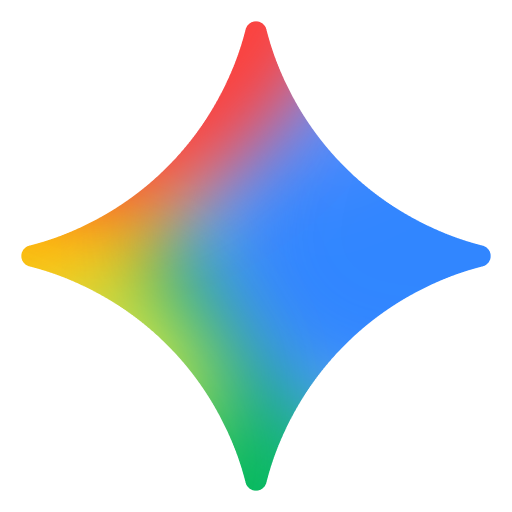
\includegraphics[width=19bp]{figures/overview/gemini.png}%
}\newcommand{\QwenLogo}{%
  \includegraphics[width=50bp]{figures/overview/qwen.jpg}%
}\newcommand{\UnslothLogo}{%
  
\includegraphics[width=50bp]{figures/overview/unsloth.png}%
}\newcommand{\DatasetReconstructImage}{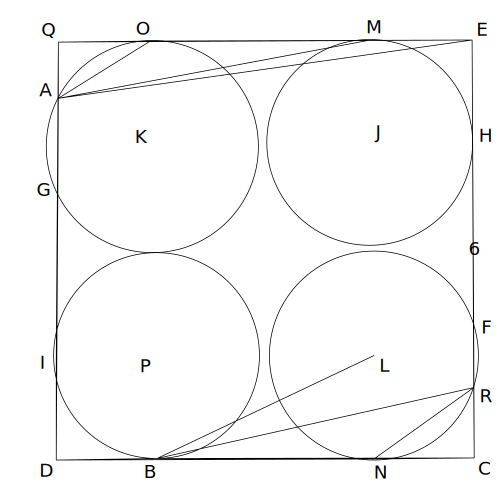
\includegraphics[width=6cm]{dataset-reconstruct-example.png}}

\begin{document}
\begin{titlepage}
\centering
\vspace*{1.8cm}
{\large\sffamily DAT391m\par}
\begin{tikzpicture}[remember picture,overlay]
\node[align=center,text width=\textwidth,inner sep=0pt] at (current page.center) {
{\LARGE\bfseries K-12 Mathematical Diagrams with TikZ:}\\[.35cm]
{\LARGE\bfseries Generate, Edit \& Reconstruct}
};
\end{tikzpicture}\par
\vspace{14cm}
{\large\bfseries Thành viên dự án\par}
\vspace{.6cm}
\begin{tabular}{@{}lcc@{}}
\toprule
\textbf{Họ và tên} & \textbf{Roll number} \\
\midrule
Hoàng Hồng Quân & \makebox[3cm]{HE195052} \\[6pt]
Nguyễn Đình Dũng & \makebox[3cm]{HE} \\
\bottomrule
\end{tabular}\par
\vfill
{\large Hà Nội, tháng 10 năm 2026\par}
\end{titlepage}
\pagenumbering{roman}
\tableofcontents
\clearpage
\pagenumbering{arabic}
\section{Introduction}
\label{sec:introduction}
\subsection{Motivation}
Hình vẽ toán học giúp người đọc nhận diện đối tượng, theo dõi quan hệ giữa các điểm và hiểu cấu hình của bài toán. Trong tài liệu dạy học, một hình thường cần được tái sử dụng ở nhiều kích thước, bổ sung đường phụ hoặc điều chỉnh theo một đề bài khác. Ảnh raster giữ lại hình thức hiển thị nhưng không cung cấp trực tiếp cấu trúc để thực hiện những thay đổi này. Việc chuyển hình sang mã nguồn có thể chỉnh sửa vì vậy là một bước quan trọng trong số hóa tài liệu toán học.

TikZ cung cấp các lệnh mô tả điểm, đường, đường tròn, nhãn và phép biến đổi; mã được biên dịch thành vector graphics và có thể tiếp tục chỉnh sửa trong môi trường \LaTeX. AutomaTikZ đã sử dụng TikZ làm biểu diễn đầu ra cho sinh hình khoa học từ văn bản \cite{automat}. Với hình toán học phổ thông, lợi ích của mã nguồn không chỉ nằm ở chất lượng xuất bản: các đối tượng và quan hệ trong hình còn cần được giữ đúng khi người dùng thay đổi cấu hình hoặc bổ sung một phép dựng.

Khó khăn nằm ở việc kết hợp ba yêu cầu: hiểu dữ kiện toán học, lựa chọn thông tin cần thể hiện và hiện thực hóa thông tin đó thành mã TikZ có thể biên dịch. Hai hình có thể khác tọa độ và hình dạng nhưng cùng thỏa một hệ dữ kiện. Ngược lại, một hình gần giống ảnh tham chiếu vẫn có thể đặt sai chân đường cao hoặc sử dụng sai bán kính đường tròn. Do đó, chất lượng đầu ra cần được xem xét đồng thời về cấu trúc toán học, nội dung và khả năng đọc.

\subsection{Objectives and scope}
Dự án \emph{K-12 Mathematical Diagrams with TikZ: Generate, Edit \& Reconstruct} nghiên cứu một quy trình tạo và đánh giá mã TikZ cho ba tác vụ có liên hệ: Generate tạo hình từ yêu cầu bằng văn bản; Edit thay đổi một hình TikZ đang có; Reconstruct khôi phục hình từ ảnh nguồn. Đầu ra chung là mã TikZ có thể biên dịch, chỉnh sửa và tái sử dụng. Mặc dù tên dự án sử dụng K-12, phạm vi dữ liệu trong báo cáo này giới hạn ở hình học lớp 6--12.

Mục tiêu thứ nhất là xây dựng các cặp input--target có nguồn toán học rõ ràng, trong đó yêu cầu vẽ xác định được đối tượng, quan hệ và phạm vi cần thể hiện. Mục tiêu thứ hai là giữ generation trực tiếp trên TikZ, đồng thời sử dụng biểu diễn quan sát sau thực thi để kiểm tra đầu ra. Mục tiêu thứ ba là đo riêng Compile rate, Mathematical correctness, Content coverage và Visual readability, nhằm phân biệt lỗi cú pháp, lỗi quan hệ, thiếu nội dung và lỗi trình bày.

Báo cáo trình bày cơ sở nghiên cứu, định nghĩa tác vụ, quy trình chuẩn bị dữ liệu và methodology đánh giá đã triển khai. Các lập luận hình học làm rõ vì sao một cấu hình hợp lệ không cần khớp tọa độ với target. Thiết kế thực nghiệm xác định cách sử dụng dữ liệu và các chỉ số để so sánh mô hình; báo cáo không suy ra hiệu năng mô hình từ khả năng biên dịch hoặc từ ví dụ minh họa.

\section{Related Work}
\label{sec:related-work}

\subsection{Graphics program generation}
Sinh graphics programs biểu diễn hình bằng mã có thể thực thi và chỉnh sửa. Với TikZ, các nghiên cứu tập trung vào hai dạng input: mô tả văn bản và ảnh. AutomaTikZ học ánh xạ caption--TikZ từ dữ liệu ghép cặp \cite{automat}, trong khi TikZero sử dụng image representations làm cầu nối giữa hiểu văn bản và sinh chương trình, cho phép kết hợp dữ liệu chưa ghép cặp \cite{ref1}. TikZilla mở rộng hướng sinh từ văn bản bằng SFT và RL, sử dụng rendered-image feedback trong quá trình tối ưu \cite{tikzilla}. Các phương pháp này khác nhau về nguồn supervision nhưng cùng đặt graphics program là đầu ra cuối cùng.

Đối với ảnh và sketch, DeTikZify kết hợp vision encoder với language model để khôi phục TikZ, đồng thời sử dụng MCTS với compiler diagnostics và perceptual similarity để cải thiện kết quả khi inference \cite{detikzify}. GeoTikzBridge tập trung vào hình học, sử dụng image-to-TikZ và instruction-augmented data để hỗ trợ geometric perception và reasoning \cite{geobridge}. Hướng sinh từ văn bản tương ứng với Generate, còn khôi phục từ ảnh tương ứng với Reconstruct trong dự án. Việc mô hình hóa hai tác vụ riêng cho phép phân biệt lỗi diễn giải dữ kiện với lỗi nhận dạng cấu trúc từ ảnh.

\subsection{Geometric representations and mathematical diagrams}
\label{sec:geometry-ir}
Các phương pháp dựa trên biểu diễn hình học tách diễn giải yêu cầu khỏi hiện thực hóa tọa độ. MagicGeo chuyển mô tả sang formal language gồm điểm và ràng buộc, rồi sử dụng solver trước bước sinh hình có thông tin tọa độ \cite{magicgeo}. GeoLoom phát triển GeoLingua để biểu diễn hình, constructive dependencies và các điều kiện hình học, kết hợp coordinate solver và constraint-based evaluation \cite{ref3}.

Khác với các tập scientific figures tổng quát, MathemaTikZ xây dựng benchmark từ curriculum, ghép diagram với mô tả, ngữ cảnh bài toán và TikZ \cite{mathematikz}. Thí nghiệm sinh hình của công trình sử dụng 50 diagram lớp 7 và đánh giá việc bảo toàn thông tin toán học bằng phán xét binary của người chấm. Hai hướng nghiên cứu bổ sung nhau: formal representations xác định quan hệ cần thỏa, còn dữ liệu có ngữ cảnh xác định nội dung cần truyền đạt. Dự án tập trung vào dữ liệu lớp 6--12 của Việt Nam, giữ TikZ là đầu ra và sử dụng biểu diễn quan sát cho bước verification sau generation.

\subsection{Instruction-guided figure editing}
Figure editing đòi hỏi hoàn thành thay đổi được yêu cầu đồng thời bảo toàn nội dung còn lại. Edit2TikZ xây dựng benchmark từ ảnh nguồn và instruction, tổ chức thay đổi thành tám loại edit operations và đánh giá riêng edit completion với non-target preservation \cite{edit2tikz}. EdiTikZ khai thác các cặp hình có liên hệ trong revision trajectories để xây dựng DaEdiTikZ, suy ra instruction từ renders và mã, rồi huấn luyện chung reconstruction và editing trước giai đoạn RL \cite{editikz}. Một hướng tập trung vào benchmark và edit units, hướng còn lại tập trung vào supervision từ thay đổi của hình do con người tạo.

Các settings nhận ảnh nguồn phải xử lý cả khôi phục mã và thực hiện chỉnh sửa. Trong dự án, Edit nhận trực tiếp \texttt{current\_tikz} cùng instruction, nên việc chỉnh sửa được đặt trên một chương trình đã có. Sự khác biệt về input này cần được giữ khi lựa chọn dữ liệu và baselines; yêu cầu bảo toàn các đối tượng ngoài phạm vi sửa vẫn là thuộc tính chung của tác vụ.

\subsection{Diagram evaluation}
Đánh giá graphics programs thường kết hợp compilation success, độ tương đồng mã và độ tương đồng bản render \cite{detikzify,ref1}. Những thước đo này phản ánh khả năng thực thi và fidelity với tham chiếu. Đối với editing, Edit2TikZ bổ sung RestorationScore và EditCorrectnessScore, sử dụng model judge được đối chiếu với human annotations để đánh giá phần giữ nguyên và phần thay đổi \cite{edit2tikz}. MathemaTikZ sử dụng human evaluation để xác định việc bảo toàn thông tin toán học \cite{mathematikz}. Các lựa chọn này khác nhau về đơn vị và mục tiêu đánh giá, từ chất lượng toàn hình tới mức hoàn thành một phép sửa.

DiagramIR đưa việc kiểm tra quan hệ vào một pipeline gồm semantic extraction và rule-based verification: LLM chuyển TikZ sang IR có schema, sau đó các checks đánh giá thực thể và quan hệ trong IR \cite{ref2}. IR ở đây được xây dựng từ output, khác với formal representations làm input cho coordinate solver trong MagicGeo và GeoLoom \cite{magicgeo,ref3}. Dự án sử dụng PDF/PGF để xác lập bằng chứng sau thực thi và tính riêng Compile rate, Mathematical correctness, Content coverage, Visual readability. Cách tiếp cận này đặt trọng tâm vào các quan hệ và đối tượng quan sát được thay vì yêu cầu output khớp tọa độ hoặc chuỗi lệnh của target.

Bảng~\ref{tab:related-work} tổng hợp input và cơ chế của các hướng nghiên cứu trên.



\begin{table}[tbp]
\centering
\small
\caption{Các hướng nghiên cứu liên quan tới Generate, Edit, Reconstruct và evaluation. Các mô tả là tổng hợp của báo cáo từ những công trình được trích dẫn.}
\label{tab:related-work}
\renewcommand{\arraystretch}{1.15}
\begin{tabularx}{\linewidth}{@{}>{\raggedright\arraybackslash}p{.24\linewidth} >{\raggedright\arraybackslash}p{.22\linewidth} >{\raggedright\arraybackslash}X@{}}
\toprule
\textbf{Công trình} & \textbf{Input / trọng tâm} & \textbf{Cơ chế và ý nghĩa đối với dự án} \\
\midrule
MathemaTikZ \cite{mathematikz} & Mô tả, ngữ cảnh toán học & Benchmark theo curriculum; target gắn với nội dung bài toán. \\
AutomaTikZ; TikZilla \cite{automat,tikzilla} & Text-to-TikZ & Sinh mã trực tiếp; supervision ghép cặp và rendering-aware training. \\
TikZero \cite{ref1} & Text-guided synthesis & Image representations kết nối các nguồn dữ liệu chưa ghép cặp. \\
MagicGeo; GeoLoom \cite{magicgeo,ref3} & Mô tả hình học & Formal representation và coordinate solver; tách dữ kiện khỏi hiện thực hóa tọa độ. \\
DeTikZify; GeoTikzBridge \cite{detikzify,geobridge} & Image/sketch-to-TikZ & Học khôi phục chương trình; search hoặc dữ liệu hình học hỗ trợ perception. \\
Edit2TikZ; EdiTikZ \cite{edit2tikz,editikz} & Ảnh và yêu cầu sửa & Edit units hoặc revision trajectories; phân biệt edit application và preservation. \\
DiagramIR \cite{ref2} & TikZ-to-IR & Semantic extraction bằng LLM, sau đó kiểm tra theo quy tắc. \\
\bottomrule
\end{tabularx}
\end{table}

\section{Methodology}
\label{sec:methodology}
\subsection{Overview}
\label{sec:overview}
\begin{figure}[p]
\centering
\begin{tikzpicture}[x=1cm,y=1cm,
font=\sffamily\fontsize{8.5}{11}\selectfont,
every node/.style={text=textMain,align=center,inner sep=3pt},
panel/.style={draw=black!28,fill=black!1,rounded corners=8pt,line width=.8pt},
phase/.style={anchor=west,font=\sffamily\bfseries\fontsize{10}{12}\selectfont},
tile/.style={draw=borderPrimary,fill=white,rounded corners=3pt,line width=.65pt,inner sep=7pt},
arrow/.style={-{Stealth[length=5pt,width=4pt]},draw=arrowColor,line width=1pt,rounded corners=3pt},
route/.style={arrow,draw=black!45,line width=1.15pt},
muted/.style={text=textLight,font=\sffamily\fontsize{8}{10}\selectfont}]
\path[use as bounding box] (0,0) rectangle (16.3,-15.15);
\filldraw[panel] (0,0) rectangle (7.75,-3.35);
\filldraw[panel] (8.1,0) rectangle (16.3,-3.35);
\node[phase] at (.3,-.4) {(i) Textbook parsing};
\node[phase] at (8.4,-.4) {(ii) ToC parsing and manual selection};
\begin{scope}[shift={(.65,-1.05)}]
\filldraw[draw=borderPrimary,fill=bgPrimary] (.12,-.12) rectangle (1.12,-1.3);
\filldraw[draw=borderPrimary,fill=white] (0,0) rectangle (1,-1.18);
\draw[borderPrimary] (.15,-.2)--(.82,-.2) (.15,-.35)--(.7,-.35);
\draw[probeAccent,line width=.7pt] (.2,-.95)--(.48,-.55)--(.82,-.95)--cycle;
\end{scope}
\node at (1.23,-2.8) {SGK / SGV\\Grades 6--12};
\node[fill=white,inner sep=4pt] at (3.15,-1.28) {\MinerULogo};
\node[muted] at (3.15,-2.32) {OCR + layout};
\node[tile] (pages) at (5.85,-1.8) {\textbf{Parsed pages}\\[3pt]Markdown\\Formulas + crops\\Page references};
\draw[arrow] (1.95,-1.8)--(pages.west);
\node[anchor=west] (chapter) at (8.5,-1.18) {\textbf{Chapter}};
\node[anchor=west] (lesson) at (8.9,-1.77) {Lesson};
\node[anchor=west] (problem) at (9.3,-2.36) {Problem};
\draw[borderPrimary] (8.67,-1.43)|-(8.9,-1.77);
\draw[borderPrimary] (9.07,-2.02)|-(9.3,-2.36);
\node[tile,fill=bgPrimary] (selected) at (14,-1.85)
{\textbf{Geometry problems}\\[3pt]Statement + subquestions\\Linked source figure};
\draw[arrow] (10.8,-1.85)--(selected.west);
\node[muted] at (11.42,-1.13) {Rule-based\\ToC};
\node[muted] at (14,-2.95) {Selected by manual review};
\draw[route] (7.75,-1.8)--(8.1,-1.8);

\filldraw[panel] (0,-3.8) rectangle (16.3,-9.5);
\node[phase] at (.3,-4.2) {(iii) Synthetic TikZ construction};
\node[fill=white,inner sep=2pt] at (10.5,-4.48) {\GeminiLogo};
\node[anchor=west,font=\sffamily\bfseries\fontsize{9}{11}\selectfont] at (11,-4.48) {Gemini 3.8 Flash High};
\draw[route] (14,-3.35)--(14,-3.8);
\node[tile,fill=bgPrimary,text width=3.15cm,minimum width=3.65cm,
minimum height=1.55cm,inner sep=5pt,
font=\sffamily\fontsize{8}{10}\selectfont] (author) at (2.35,-5.975)
{\textbf{Generate / Edit}\\[3pt]
Givens $\rightarrow$ instruction\\
+ current TikZ for Edit};
\node[tile,fill=bgProbe!45,text width=3.15cm,minimum width=3.65cm,
minimum height=1.55cm,inner sep=5pt,
font=\sffamily\fontsize{8}{10}\selectfont,below=2mm of author] (reconstruct)
{\textbf{Reconstruct}\\[3pt]
Diagram image};

\filldraw[draw=borderPrimary!60,fill=bgPrimary!35,rounded corners=5pt]
(4.85,-5.2) rectangle (12.5,-8.85);
\node[font=\sffamily\bfseries] at (8.68,-5.58) {ReAct drawing harness};
\node[tile,minimum width=2.3cm] (reason) at (6.55,-6.85)
{\textbf{TikZ generation}\\Model reasoning};
\node[tile,minimum width=2.5cm,fill=bgProbe!45,font=\sffamily\fontsize{8}{10}\selectfont] (render) at (10.55,-6.85)
{\textbf{Rendering tools}\\Compile\\Label collision repair\\Relation-mark placement};
\coordinate (inputjoin) at (4.55,-6.85);
\draw[draw=arrowColor,line width=1pt,rounded corners=3pt]
  (author.east)-|(inputjoin) (reconstruct.east)-|(inputjoin);
\draw[arrow] (inputjoin)--(reason.west);
\draw[arrow] (reason.east)--node[above,muted]{Code}(render.west);
\draw[arrow] (render.south)--(10.55,-8.17)--(6.55,-8.17)--(reason.south);
\node[muted] at (8.55,-8.57) {Visual feedback + compiler diagnostics};


\node[font=\sffamily\bfseries] at (14.45,-5.58) {Generated diagram};
\begin{scope}[shift={(13.4,-7.6)}]
\coordinate (oa) at (.5,1.25);
\coordinate (ob) at (0,0);
\coordinate (oc) at (2,0);
\coordinate (om) at (1,0);
\draw[borderAccent,line width=.85pt] (oa)--(ob)--(oc)--cycle (oa)--(om);
\foreach \point/\pos/\lab in {oa/above/A,ob/below left/B,oc/below right/C,om/below/M}
  \node[\pos,inner sep=2pt,font=\sffamily\fontsize{8}{9}\selectfont] at (\point) {$\lab$};
\draw[probeAccent] (.47,-.07)--(.53,.07) (1.47,-.07)--(1.53,.07);
\end{scope}
\node[muted] at (14.45,-8.65) {TikZ + render};
\draw[arrow] (render.east)--(13.15,-6.85);
\draw[route] (14.45,-9.5)--(14.45,-9.77)--(2.4,-9.77)--(2.4,-10.05);

\filldraw[panel] (0,-10.05) rectangle (4.85,-14.45);
\filldraw[panel] (5.2,-10.05) rectangle (10.05,-14.45);
\filldraw[panel] (10.4,-10.05) rectangle (16.3,-14.45);
\node[phase] at (.3,-10.45) {(iv) Data curation};
\node[phase] at (5.5,-10.45) {(v) Fine-tuning};
\node[phase] at (10.7,-10.45) {(vi) Evaluation};

\node[font=\sffamily\fontsize{8}{10}\selectfont,inner sep=2pt]
(pairs) at (2.4,-11.18) {Generate / Edit / Reconstruct};
\node[tile,fill=bgProbe,minimum width=3.55cm,inner sep=4pt,
font=\sffamily\fontsize{8}{10}\selectfont,below=3mm of pairs] (review)
{\textbf{Quality review}\\Mathematical consistency\\Instruction alignment};
\draw[arrow] (pairs.south)--(review.north);
\node[muted,inner sep=1pt,below=1.5mm of review] (split) {Problem-level split};
\node[tile,fill=bgPrimary,inner sep=4pt,below=1.5mm of split,xshift=-1.42cm] (train) {Train};
\node[tile,inner sep=4pt,below=1.5mm of split,xshift=.07cm] {Validation};
\node[tile,inner sep=4pt,below=1.5mm of split,xshift=1.48cm] (test) {Test};

\node[fill=white,inner sep=3pt] at (6.42,-11.25) {\QwenLogo};
\node[fill=white,inner sep=3pt] at (8.72,-11.25) {\UnslothLogo};
\node[tile,fill=bgPrimary!55,minimum width=3.5cm] (sft) at (7.63,-12.25)
{\textbf{Supervised fine-tuning}\\Qwen3.5};
\node[tile,minimum width=3.5cm] (checkpoint) at (7.63,-13.65)
{\textbf{Fine-tuned model}};
\draw[arrow] (sft.south)--(checkpoint.north);


\node[tile,minimum width=4.65cm,inner sep=5pt] (prediction) at (13.35,-11.38)
{\textbf{Model inference}\\Test input $\rightarrow$ generated TikZ};
\node[tile,fill=bgProbe,minimum width=4.65cm,inner sep=5pt,
font=\sffamily\fontsize{8}{10}\selectfont] (metrics) at (13.35,-13.2)
{\textbf{Deterministic evaluation}\\[3pt]
Compile rate\\
Mathematical correctness\\
Content coverage\\
Visual readability};
\draw[arrow] (prediction.south)--(metrics.north);

\draw[route] (4.85,-12.25)--(sft.west);
\draw[route] (checkpoint.east)--(10.22,-13.65)|-(prediction.west);
\draw[arrow,dashed] (test.south)--(3.88,-14.87)--(16.08,-14.87)|-(metrics.east);
\node[muted,fill=white,inner sep=2pt] at (9.35,-14.87) {Reference TikZ};
\end{tikzpicture}
\caption[Overview of the curriculum-grounded TikZ pipeline]{\textbf{Overview of the curriculum-grounded TikZ pipeline.} MinerU chuyển SGK/SGV thành văn bản, công thức và hình có liên kết nguồn. ToC Parser phân đoạn theo quy tắc, sau đó manual review lựa chọn các bài toán hình học. Gemini tạo instruction và sinh TikZ qua vòng lặp generate--render--revise. Các cặp dữ liệu được rà soát, chia theo bài toán nguồn và dùng cho fine-tuning Qwen3.5 với Unsloth. Output trên held-out inputs được đánh giá bằng bốn metrics. Ví dụ trung tuyến minh họa input và hình đầu ra.}
\label{fig:method-overview}
\end{figure}
Chúng tôi xây dựng một pipeline từ tài liệu toán học phổ thông đến dữ liệu huấn luyện cho ba tác vụ Generate, Edit và Reconstruct (Hình~\ref{fig:method-overview}). Pipeline gồm sáu giai đoạn: phân tích tài liệu bằng OCR, phân đoạn theo cấu trúc mục lục và tuyển chọn bài toán, tạo dữ liệu TikZ, rà soát và tổ chức dữ liệu, supervised fine-tuning, và đánh giá tất định. Nội dung toán học được lấy từ SGK/SGV lớp 6--12 thuộc bộ \emph{Kết nối tri thức với cuộc sống}. Văn bản, công thức và hình minh họa được giữ cùng vị trí nguồn để làm căn cứ cho việc biên soạn yêu cầu vẽ và kiểm tra target.

MinerU chuyển tài liệu thành nội dung có cấu trúc \cite{mineru}; ToC Parser và manual review xác định các bài toán được đưa vào bước tạo dữ liệu. Google Gemini 3.8 Flash với thinking level \texttt{high} thực hiện biên soạn instruction và sinh mã trong drawing harness \cite{geminiflash}. Các cặp input--target được rà soát trước khi dùng cho fine-tuning Qwen3.5 bằng Unsloth \cite{qwen35,unsloth35}. Mục~\ref{sec:tasks} xác định các tác vụ; Mục~\ref{sec:document-parsing}--\ref{sec:problem-extraction} trình bày xử lý nguồn; Mục~\ref{sec:information-selection}--\ref{sec:data-curation} mô tả xây dựng và tuyển chọn dữ liệu. Giai đoạn huấn luyện và bốn metrics được trình bày lần lượt tại Mục~\ref{sec:fine-tuning} và Mục~\ref{sec:evaluation}.

\subsection{Task formulation}
\label{sec:tasks}
Chúng tôi biểu diễn đầu ra của cả ba tác vụ bằng mã TikZ có thể biên dịch và chỉnh sửa. Cách đặt bài toán dưới dạng sinh chương trình đồ họa có điều kiện đã được sử dụng cho text-to-TikZ trong AutomaTikZ \cite{automat}, image-to-TikZ trong DeTikZify \cite{detikzify}, và chỉnh sửa theo instruction trong EdiTikZ \cite{editikz}. Gọi $I$ là instruction, $Z_{\mathrm{in}}$ là mã TikZ hiện tại, $J$ là ảnh diagram và $Z$ là mã đầu ra. Các ánh xạ được xác định như sau:
\begin{equation}
\begin{aligned}
\mathrm{Generate}:&\quad I \longmapsto Z,\\
\mathrm{Edit}:&\quad (I,Z_{\mathrm{in}}) \longmapsto Z,\\
\mathrm{Reconstruct}:&\quad (I,J) \longmapsto Z.
\end{aligned}
\end{equation}
Với Generate, $I$ mô tả đầy đủ các đối tượng, quan hệ và phép dựng cần thể hiện. Với Edit, $I$ xác định thay đổi trên $Z_{\mathrm{in}}$; phần hình không thuộc phạm vi thay đổi được bảo toàn. Với Reconstruct, $J$ cung cấp cấu hình cần tái tạo, còn $I$ là yêu cầu khôi phục hình. Mô hình cần tái hiện các đối tượng, kết nối và ký hiệu quan sát được trong ảnh bằng mã TikZ.

Mỗi mẫu có một target $Z^\star$ được chuẩn bị ngoại tuyến để làm đầu ra supervision và tham chiếu đánh giá. Khi thực hiện tác vụ, mô hình chỉ nhận các thành phần đầu vào tương ứng trong ánh xạ trên. Target, quyết định duyệt và điểm đánh giá không được đưa vào context sinh mã.

\subsection{Textbook document parsing}
\label{sec:document-parsing}
Tài liệu nguồn gồm SGK và SGV Toán lớp 6--12 thuộc bộ \emph{Kết nối tri thức với cuộc sống}. Chúng tôi sử dụng MinerU để nhận dạng văn bản, công thức và bố cục trang, đồng thời trích xuất hình minh họa từ PDF \cite{mineru}. Đầu ra được tổ chức thành văn bản Markdown, thông tin layout và các image crops. Liên kết giữa nội dung trích xuất với trang và khối nguồn được giữ lại để hỗ trợ đối chiếu khi phát biểu chứa ký hiệu mơ hồ hoặc phụ thuộc vào hình.

Cấu trúc sau OCR được chuẩn hóa theo quy tắc trình bày của từng cuốn sách. Các heading và khối nội dung được gán vai trò dựa trên dấu hiệu bố cục của trang in. Đối với SGK, các vai trò phân biệt bài học, mục kiến thức, ví dụ, luyện tập, vận dụng và bài tập. Đối với SGV, các vai trò phân biệt đơn vị dạy học, mục tiêu và hướng dẫn giảng dạy. Sự phân biệt này được giữ trong dữ liệu đầu ra để bước tuyển chọn có thể xác định đâu là phát biểu bài toán và đâu là phần giải thích hoặc hướng dẫn.

\subsection{Rule-based ToC parsing and problem selection}
\label{sec:problem-extraction}
ToC Parser sử dụng các quy tắc về cấp heading và vai trò nội dung để phân đoạn tài liệu theo chương, bài học và mục. Các khối văn bản, công thức và hình được gom theo vùng nội dung tương ứng, đồng thời giữ thứ tự đọc và vị trí nguồn. Bước này tạo các đơn vị tài liệu để rà soát, chưa quyết định đơn vị nào đủ điều kiện trở thành một mẫu huấn luyện.

Chúng tôi tuyển chọn các bài toán hình học bằng manual review. Đơn vị tuyển chọn là một ví dụ, luyện tập hoặc bài tập hoàn chỉnh, bao gồm các tiểu ý và ngữ cảnh cần thiết để xác định giả thiết, đối tượng và phép dựng. Người rà soát đối chiếu phát biểu với hình đi kèm và giữ những bài có thể xác định rõ nội dung cần thể hiện. Các ký hiệu hoặc nhánh cấu hình chưa xác định được được giữ lại để rà soát tiếp, trước khi chuyển sang biên soạn instruction. Khi SGV cung cấp ngữ cảnh bổ sung, nội dung này vẫn được phân biệt với giả thiết của đề bài.

Mỗi bài toán được gắn lớp học, sách, vị trí văn bản, trang và hình nguồn. Những bản ghi xuất phát từ cùng một bài toán được liên kết bằng source family. Định danh này được truyền qua các bước tạo dữ liệu và curation để truy xuất nguồn và kiểm soát việc chia train, validation và test.

\subsection{Mathematical givens and information selection}
\label{sec:information-selection}
Instruction được biên soạn từ mathematical givens và phạm vi dựng hình của bài toán đã tuyển chọn. Các phương pháp như MagicGeo và GeoLoom sử dụng ràng buộc hình học để xác định tọa độ từ mô tả ngôn ngữ \cite{magicgeo,ref3}. Trong phương pháp của chúng tôi, các định nghĩa và quan hệ cần dựng được diễn đạt trực tiếp trong instruction; mô hình sinh mã TikZ từ instruction này. Việc biên soạn phân biệt ba thành phần: dữ kiện có trong nguồn, quan hệ cần thỏa khi dựng hình, và thông tin cần truyền đạt qua nét vẽ, nhãn hoặc ký hiệu.

Chẳng hạn, yêu cầu dựng trung tuyến $AM$ của tam giác $ABC$ cần xác định $M$ là trung điểm của $BC$ và yêu cầu vẽ đoạn $AM$. Định nghĩa trung điểm quyết định vị trí phụ thuộc của $M$, còn yêu cầu vẽ quyết định sự hiện diện của đoạn $AM$ trong hình. Tọa độ cụ thể của các đỉnh có thể thay đổi trong những cấu hình thỏa giả thiết. Instruction chỉ giữ các điều kiện tọa độ hoặc độ dài khi chúng là một phần của nội dung toán học cần thể hiện.

Đối với các phép dựng phụ, instruction xác định đối tượng tham chiếu, điều kiện dựng và nhánh cấu hình khi có nhiều nghiệm. Kết luận cần chứng minh được phân biệt với giả thiết để tránh đưa kết quả bài toán thành điều kiện đầu vào. Các relation marks được lựa chọn theo thông tin cần truyền đạt; sự tồn tại của một quan hệ hình học không tự động yêu cầu thêm một dấu riêng cho mọi vị trí có quan hệ đó.

\subsection{Synthetic TikZ construction}
\label{sec:drawing-workflow}
Giai đoạn này tạo các cặp dữ liệu ứng viên từ input theo từng tác vụ. Google Gemini 3.8 Flash với thinking level \texttt{high} được sử dụng cho instruction authoring và sinh TikZ \cite{geminiflash}. Với Generate, bước authoring diễn đạt các mathematical givens thành yêu cầu vẽ tự chứa. Với Edit, bước này xác định thay đổi trên một bản TikZ có sẵn và giữ liên kết với cấu hình ban đầu. Với Reconstruct, ảnh diagram là dữ liệu điều kiện để chuẩn bị target tương ứng. Ảnh nguồn được giữ nguyên trong cặp dữ liệu; phần TikZ là biểu diễn cần tái tạo.

Drawing harness tổ chức việc sinh và sửa mã theo vòng lặp ReAct, trong đó mô hình xen kẽ suy luận với hành động gọi công cụ và sử dụng kết quả công cụ cho bước tiếp theo \cite{react}. Ở mỗi vòng, mô hình đề xuất mã TikZ; công cụ render biên dịch mã trong wrapper thống nhất và trả lại ảnh cùng compiler diagnostics. Mô hình sử dụng phản hồi này để sửa mã hoặc kết thúc. Số lần gọi được giới hạn bởi harness; những lượt không tạo được kết quả hợp lệ trong ngân sách được ghi nhận là thất bại. Cách sử dụng compiler feedback để sửa mã cũng xuất hiện trong pipeline chuẩn bị dữ liệu của TikZilla \cite{tikzilla}.

Khâu hoàn thiện bản vẽ xử lý khoảng cách giữa nhãn và nét vẽ, đồng thời bố trí relation marks trên các đối tượng tương ứng. Các điều chỉnh trình bày giữ nguyên các quan hệ dựng hình đã xác định. Sau mỗi lần sửa, mã được biên dịch lại để phản hồi gắn với đúng phiên bản TikZ. Harness lưu input, mã cuối, render và lịch sử xử lý; các artifacts này được chuyển sang bước curation để kiểm tra sự phù hợp giữa yêu cầu và hình thực tế.

\subsection{Data curation}
\label{sec:data-curation}
Data curation chuyển các cặp ứng viên thành dữ liệu supervision đã được rà soát. Với mỗi cặp, người rà soát kiểm tra sự phù hợp giữa input và target, các quan hệ toán học bắt buộc, phạm vi nội dung và khả năng đọc của render. Generate được đối chiếu với instruction và các mathematical givens; Edit được kiểm tra cả thay đổi yêu cầu lẫn phần nội dung cần bảo toàn; Reconstruct được đối chiếu với ảnh đầu vào. Mẫu có sai lệch được sửa và rà soát lại hoặc loại khỏi tập sử dụng. Biên dịch thành công là điều kiện thực thi, không thay thế kiểm tra nội dung toán học.

Quyết định chấp nhận được gắn với đúng input, target TikZ và render đã xem xét. Khi một thành phần thay đổi, cặp dữ liệu cần được rà soát lại. Provenance lưu quan hệ với bài toán nguồn và các phiên bản trước, đồng thời phân biệt kết quả sinh ban đầu, sửa bằng công cụ, sửa có hỗ trợ mô hình và sửa thủ công. Nhờ đó, việc sử dụng target cho huấn luyện không đồng nhất thành công của bước sinh mã với chất lượng của dữ liệu đã tuyển chọn.

Dữ liệu được chia theo source family: mọi biến thể, bản sao và cặp Generate/Edit có chung bài toán nguồn thuộc cùng một split. Nếu một mẫu kết hợp nhiều nguồn, các nguồn liên quan được gom trong cùng nhóm chia dữ liệu. Train split cung cấp supervision; validation split phục vụ lựa chọn cấu hình và checkpoint; test split được dành cho đánh giá cuối. Các mẫu validation và test không được dùng làm ví dụ authoring hoặc repair để mở rộng train split.

\subsection{Supervised fine-tuning with Qwen3.5 and Unsloth}
\label{sec:fine-tuning}
Chúng tôi xây dựng quy trình supervised fine-tuning (SFT) trên Qwen3.5, sử dụng khả năng xử lý văn bản và hình ảnh của họ mô hình này \cite{qwen35}. Unsloth cung cấp công cụ fine-tuning cho cả đầu vào text và vision \cite{unsloth35}. Mỗi mẫu được chuyển thành chuỗi hội thoại theo chat template của checkpoint: phần input chứa instruction và các thành phần theo tác vụ, còn assistant completion chứa target TikZ đã duyệt. Generate sử dụng văn bản, Edit bổ sung mã hiện tại, và Reconstruct bổ sung ảnh diagram. Cả ba tác vụ dùng chung định dạng đầu ra TikZ.

Gọi $\mathcal{D}_{\mathrm{train}}=\{(X_i,Z_i^\star)\}_{i=1}^{N}$ là tập huấn luyện, trong đó $X_i$ là input và $Z_i^\star=(z_{i1}^\star,\ldots,z_{iT_i}^\star)$ là chuỗi token của target. Mục tiêu huấn luyện là negative log-likelihood của target có điều kiện theo input, tương ứng với mục tiêu autoregressive được dùng trong text-to-TikZ SFT \cite{tikzilla}:
\begin{equation}
\mathcal{L}_{\mathrm{SFT}}(\theta)=
-\frac{1}{N}
\sum_{i=1}^{N}
\sum_{t=1}^{T_i}
\log p_\theta(z_{it}^\star\mid X_i,z_{i,<t}^\star).
\end{equation}
Loss được tính trên assistant completion. Các token của instruction, mã đầu vào và biểu diễn ảnh cung cấp điều kiện cho dự đoán và được loại khỏi phần tính loss. Các mẫu huấn luyện giữ nguyên target hoàn chỉnh để tránh tạo supervision từ mã TikZ bị cắt mất phần kết thúc.

Thiết kế fine-tuning sử dụng Low-Rank Adaptation (LoRA), giữ cố định trọng số nền và học các cập nhật hạng thấp \cite{lora}. Unsloth thực hiện việc gắn và tối ưu các adapters cho Qwen3.5 \cite{unsloth35}. Việc lựa chọn cấu hình và checkpoint dựa trên validation split; mô hình được chọn sau đó sinh output cho test inputs. Các output này được chuyển sang phương pháp đánh giá tại Mục~\ref{sec:evaluation}, với cùng điều kiện biên dịch và ngân sách sinh/sửa được quy định trong protocol thực nghiệm.

\subsection{Evaluation}
\label{sec:evaluation}
\subsubsection{Evaluation objectives and principles}

Đánh giá hình vẽ toán học cần phân biệt khả năng thực thi mã, tính đúng của các quan hệ hình học, mức độ đầy đủ của nội dung và khả năng đọc hình. Các công trình về sinh TikZ như TikZero sử dụng nhiều thước đo cho độ tương đồng hình ảnh và mã nguồn \cite{ref1}. Tuy nhiên, đối với hình học, cùng một hệ quan hệ có thể được biểu diễn bằng nhiều cấu hình khác nhau. Vì vậy, độ giống nhau về hình dạng hoặc chuỗi lệnh không đủ để xác định tính đúng toán học.

Phương pháp này đánh giá hình vẽ thông qua các đối tượng và quan hệ quan sát được sau khi thực thi TikZ. Cách tách biểu diễn hình học khỏi phép kiểm tra cũng được sử dụng trong DiagramIR, nơi LLM chuyển TikZ sang một biểu diễn trung gian để áp dụng các kiểm tra theo quy tắc \cite{ref2}. Ở đây, biểu diễn được trích xuất trực tiếp từ PDF và thông tin thực thi PGF; việc tính điểm sử dụng các phép kiểm tra tất định.

Với mã tham chiếu $T=\texttt{target\_tikz}$ và mã do mô hình sinh $O=\texttt{output\_tikz}$, hàm đánh giá trả về

\begin{equation}
\operatorname{Eval}(T,O)=(C,M,K,V),
\qquad C\in\{0,1\},\quad M,K,V\in[0,100].
\end{equation}

Bốn thành phần lần lượt là \textbf{Compile}, \textbf{Mathematical correctness}, \textbf{Content coverage} và \textbf{Visual readability}. Target xác định các quan hệ và nội dung cần đối chiếu; bộ đánh giá không yêu cầu tọa độ tuyệt đối hoặc cách viết lệnh của output trùng với target. Cùng một phương pháp được áp dụng cho Generate, Edit và Reconstruct.

\subsubsection{Representation extraction from execution outputs}

Hai mã TikZ được xử lý bằng cùng wrapper và compiler để thu được các biểu diễn quan sát $X_T$ và $X_O$. Mỗi biểu diễn gồm các điểm có định danh và vị trí, đường đã vẽ, kiểu nét, đường tròn, nhãn văn bản và vùng mực của ký tự. Hình~\ref{fig:evaluation-pipeline} mô tả vai trò của hai nguồn bằng chứng trong quá trình này.

\begin{figure}[tbp]
\centering
\resizebox{\linewidth}{!}{%
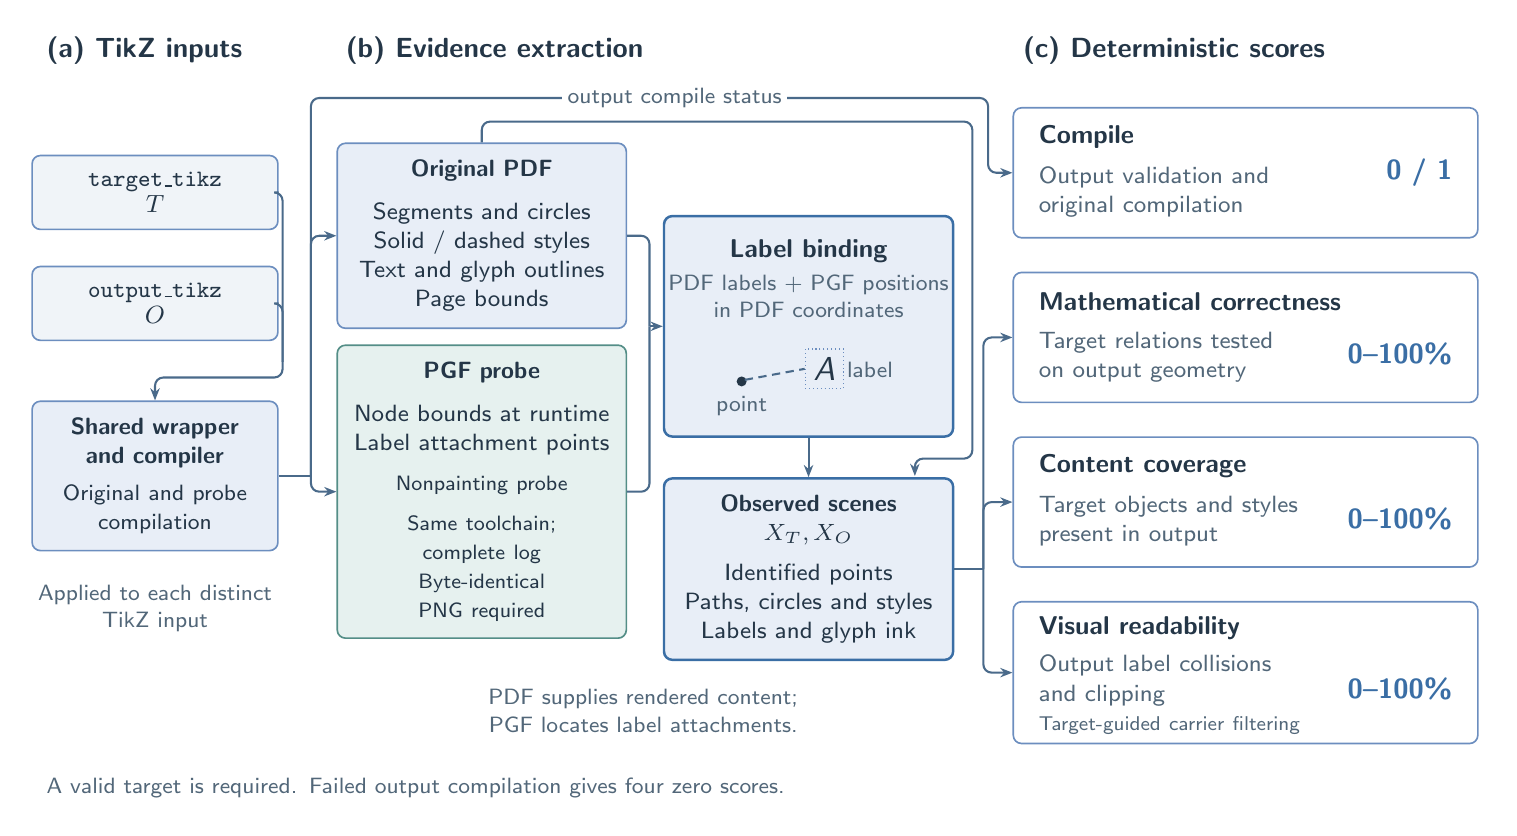
\begin{tikzpicture}
\node[heading] at (0,10.5) {(a) TikZ inputs};
\node[heading] at (3.8,10.5) {(b) Evidence extraction};
\node[heading] at (12.4,10.5) {(c) Deterministic scores};

\node[input] (target) at (1.5,8.7) {\texttt{target\_tikz}\\[-1pt]{\small $T$}};
\node[input,below=.45cm of target] (output) {\texttt{output\_tikz}\\[-1pt]{\small $O$}};
\node[card,text width=2.7cm,minimum height=1.5cm] (compiler) at (1.5,5.1)
  {\textbf{Shared wrapper}\\\textbf{and compiler}\\[4pt]
   {\footnotesize Original and probe\\compilation}};
\coordinate (inputjoin) at (3.12,6.55);
\draw[wire] (target.east) -- (3.12,8.7) -- (inputjoin);
\draw[wire] (output.east) -- (inputjoin |- output.east) -- (inputjoin);
\draw[flow] (inputjoin) -- (3.12,6.35) -| (compiler.north);
\node[note,text width=3cm,below=.3cm of compiler] {Applied to each distinct\\TikZ input};

\node[evidence] (pdf) at (5.65,8.15) {
  \textbf{Original PDF}\\[5pt]
  Segments and circles\\
  Solid / dashed styles\\
  Text and glyph outlines\\
  Page bounds
};
\node[evidence,fill=bgProbe,draw=probeAccent,minimum height=3.0cm] (probe) at (5.65,4.9) {
  \textbf{PGF probe}\\[5pt]
  Node bounds at runtime\\
  Label attachment points\\[4pt]
  {\fontsize{7.5}{9}\selectfont Nonpainting probe}\\[4pt]
  {\fontsize{7.5}{9}\selectfont Same toolchain; complete log}\\
  {\fontsize{7.5}{9}\selectfont Byte-identical PNG required}
};
\coordinate (compilex) at (3.48,0);
\coordinate (compilefork) at (compilex |- compiler.east);
\draw[wire] (compiler.east) -- (compilefork);
\draw[flow] (compilefork) |- (pdf.west);
\draw[flow] (compilefork) |- (probe.west);

\node[merge,minimum height=2.8cm] (binding) at (9.8,7.0) {};
\node[title,anchor=center] at (9.8,7.96) {Label binding};
\node[note] at (9.8,7.38) {PDF labels + PGF positions\\in PDF coordinates};
\fill[textMain] (8.95,6.3) circle[radius=1.8pt];
\node[note] at (8.95,5.99) {point};
\node[draw=borderPrimary,densely dotted,inner sep=3pt,
  font=\sffamily\itshape\fontsize{12}{12}\selectfont,text=textMain] (glyph) at (10.0,6.46) {A};
\draw[wire,densely dashed] (8.99,6.32) -- (glyph.west);
\node[note] at (10.58,6.45) {label};

\coordinate (evidencejoin) at (7.78,7.0);
\draw[wire] (pdf.east) -- (7.78,8.15) -- (evidencejoin);
\draw[wire] (probe.east) -- (7.78,4.9) -- (evidencejoin);
\draw[flow] (evidencejoin) -- (binding.west);

\node[merge,minimum height=2.2cm,below=.5cm of binding] (scene) {
  \textbf{Observed scenes}\\$X_T,X_O$\\[4pt]
  Identified points\\
  Paths, circles and styles\\
  Labels and glyph ink
};
\draw[flow] (binding.south) -- (scene.north);
\draw[flow] (pdf.north) -- (5.65,9.6) -- (11.88,9.6)
  -- (11.88,5.32) -- (11.15,5.32) -- (11.15,5.1);
\node[note,text width=7.5cm] at (7.7,2.12)
  {PDF supplies rendered content; PGF locates label attachments.};

\node[metric] (compile) at (15.35,8.95) {};
\node[title] at ([xshift=6pt,yshift=13pt]compile.west) {Compile};
\node[detail,text width=4.5cm] at ([xshift=6pt,yshift=-7pt]compile.west)
  {Output validation and\\original compilation};
\node[score] at ([xshift=-6pt]compile.east) {0 / 1};

\node[metric,below=.42cm of compile] (math) {};
\node[title] at ([xshift=6pt,yshift=13pt]math.west) {Mathematical correctness};
\node[detail,text width=4.4cm] at ([xshift=6pt,yshift=-7pt]math.west)
  {Target relations tested\\on output geometry};
\node[score] at ([xshift=-6pt,yshift=-6pt]math.east) {0--100\%};

\node[metric,below=.42cm of math] (coverage) {};
\node[title] at ([xshift=6pt,yshift=13pt]coverage.west) {Content coverage};
\node[detail,text width=4.35cm] at ([xshift=6pt,yshift=-7pt]coverage.west)
  {Target objects and styles\\present in output};
\node[score] at ([xshift=-6pt,yshift=-6pt]coverage.east) {0--100\%};

\node[metric,minimum height=1.8cm,below=.42cm of coverage] (readability) {};
\node[title] at ([xshift=6pt,yshift=16pt]readability.west) {Visual readability};
\node[detail,text width=4.25cm] at ([xshift=6pt,yshift=-8pt]readability.west)
  {Output label collisions\\and clipping\\
   {\fontsize{7.2}{9}\selectfont Target-guided carrier filtering}};
\node[score] at ([xshift=-6pt,yshift=-6pt]readability.east) {0--100\%};

\draw[flow] (compilefork) -- (3.48,9.9) -- (12.08,9.9) |- (compile.west);
\node[note,fill=white,inner sep=2pt] at (8.1,9.9) {output compile status};

\coordinate (forkx) at (12.02,0);
\coordinate (scenefork) at (forkx |- scene.east);
\draw[wire] (scene.east) -- (scenefork);
\draw[flow] (scenefork) |- (math.west);
\draw[flow] (scenefork) |- (coverage.west);
\draw[flow] (scenefork) |- (readability.west);

\node[note,anchor=north west,text width=18.2cm,align=left] at (0,1.38) {
  A valid target is required. Failed output compilation gives four zero scores.
};
\end{tikzpicture}
}
\caption{Tổng quan phương pháp đánh giá. (a) Hai đầu vào TikZ được biên dịch theo cùng quy trình. (b) Original PDF cung cấp nội dung đã vẽ; PGF probe cung cấp vị trí thực thi để gắn nhãn với điểm. Các nét vẽ và vùng mực ký tự được giữ trực tiếp từ PDF, còn định danh điểm được xác lập qua label binding. (c) Mathematical correctness và Content coverage đối chiếu hai biểu diễn quan sát; Visual readability chấm các nhãn của output. Compile được xác định từ trạng thái kiểm tra và biên dịch output.}
\label{fig:evaluation-pipeline}
\end{figure}

\textbf{PDF observations.} PDF cung cấp các vector paths, kiểu nét liền hoặc đứt, độ dày nét, văn bản và giới hạn trang. Các paths cho biết đoạn thẳng hoặc đường tròn nào thực sự được vẽ. Glyph outlines xác định vùng mực của chữ, phục vụ kiểm tra nhãn giao với nét vẽ, chồng lên nhãn khác hoặc bị cắt khỏi trang. Nhờ đó, sự hiện diện của đối tượng được xác định từ kết quả hiển thị.

\textbf{PGF probe và label binding.} PGF probe ghi nhận vị trí node và điểm gắn nhãn khi TikZ thực thi, không bổ sung nét vẽ. Thông tin này giải quyết sự khác biệt giữa vị trí của điểm toán học và vị trí chữ dùng để đặt tên điểm: nhãn $A$ thường được đặt lệch khỏi điểm $A$ để tránh che hình. Văn bản đọc từ PDF được ghép với vị trí ghi nhận từ PGF và quy về hệ tọa độ PDF. Probe chỉ được chấp nhận khi biên dịch thành công, có nhật ký đầy đủ, dùng cùng toolchain và tạo PNG trùng từng byte với bản gốc.

PDF và PGF có vai trò bổ sung: PDF xác định nội dung đã hiển thị; PGF hỗ trợ xác định vị trí gắn nhãn. Các vị trí này là dữ liệu cho phép kiểm tra quan hệ, không tự tạo thành một kết luận về tính đúng toán học. Một liên kết nhãn không xác định được duy nhất không được coi là bằng chứng đạt.

\subsubsection{Evaluation metrics}

\paragraph{Compile và Compile rate}

Với mẫu thứ $i$, đặt $C_i=1$ nếu output vượt qua kiểm tra đầu vào và biên dịch thành công; ngược lại $C_i=0$. Compile rate trên tập gồm $N$ mẫu là

\begin{equation}
\operatorname{CompileRate}
=\frac{100}{N}\sum_{i=1}^{N}C_i.
\end{equation}

Compile đo khả năng tạo ra một hình có thể đánh giá, không xác nhận tính đúng của hình. Nếu output không biên dịch được, cả bốn điểm của mẫu bằng 0. Target không hợp lệ hoặc lỗi hạ tầng biên dịch không được quy thành lỗi chất lượng của mô hình và cần được xử lý trước khi tổng hợp kết quả.

\paragraph{Mathematical correctness}

Mathematical correctness đo mức độ bảo toàn các quan hệ hình học được suy ra từ target. Gọi $R_T=(r_1,\ldots,r_m)$ là danh sách đơn vị quan hệ cần kiểm tra. Khi $m>0$,

\begin{equation}
M(T,O)=
\frac{100}{m}\sum_{j=1}^{m}
\mathbf 1\!\left[r_j(X_O)\text{ đạt}\right].
\end{equation}

Mỗi đơn vị có trọng số bằng nhau. Danh sách quan hệ và mẫu số được xác định từ target; việc thiếu điểm hoặc thiếu bằng chứng trong output làm các đơn vị liên quan không đạt, không làm giảm mẫu số. Các điều kiện được kiểm tra bằng sai số số học tương đối, thay vì yêu cầu tọa độ bằng nhau tuyệt đối.

\begin{table}[tbp]
\centering\small
\caption{Các đơn vị quan hệ dùng cho Mathematical correctness.}
\label{tab:relations}
\renewcommand{\arraystretch}{1.18}
\begin{tabularx}{\linewidth}{@{}>{\raggedright\arraybackslash}p{.27\linewidth} >{\raggedright\arraybackslash}X >{\raggedright\arraybackslash}p{.20\linewidth}@{}}
\toprule
Quan hệ quan sát trên target & Yêu cầu đối với output & Đơn vị tính điểm \\
\midrule
Cặp điểm có định danh & Giữ trạng thái phân biệt hoặc trùng nhau & Mỗi cặp điểm \\
Bộ ba thẳng hàng & Giữ tính thẳng hàng và quan hệ trung điểm nếu có & Mỗi bộ ba \\
Các bộ ba không thẳng hàng & Giữ tính không suy biến & Một điều kiện chung \\
Điểm thuộc đoạn đã vẽ & Giữ quan hệ thuộc đoạn và giới hạn hai đầu mút & Mỗi quan hệ \\
Hai đường chứa đoạn thẳng song song, phân biệt & Giữ tính song song và quan hệ vector bằng nhau đến dấu nếu có & Mỗi cặp đường \\
Dấu góc vuông dạng ô vuông & Các tia tương ứng vẫn vuông góc & Mỗi góc được đánh dấu \\
Đường tròn đầy đủ & Giữ các quan hệ tâm, điểm thuộc đường tròn, bán kính bằng độ dài giữa hai điểm và tiếp tuyến đã nhận diện & Một đơn vị tổng hợp cho mỗi đường tròn \\
\bottomrule
\end{tabularx}
\end{table}

Các đường tròn được ghép một-một theo quan hệ hình học. Do đó, thay đường tròn $(C,CM)$ bằng $(C,CN)$ làm sai đơn vị quan hệ tương ứng khi $CM\ne CN$, dù số lượng đường tròn không thay đổi. Tương tự, một đường cao vẫn có thể hiện diện đầy đủ nhưng không đạt Mathematical correctness nếu mất quan hệ vuông góc đã được target thể hiện.

\paragraph{Content coverage}

Content coverage đo sự hiện diện của các thành phần cần biểu diễn: định danh điểm, kết nối thẳng cực đại và đường tròn. Một kết nối cực đại là nét nối giữa các điểm có định danh sau khi gộp các đoạn con thẳng hàng cùng kiểu nét; cách chia nét thành nhiều lệnh TikZ không tạo thêm đơn vị nội dung.

Gọi $U_T$ là danh sách đơn vị nội dung của target, $c_u(X_O)\in\{0,1\}$ cho biết đơn vị $u$ hiện diện hợp lệ trong output, và $e_O$ là số đơn vị phạt cho nội dung thừa hoặc đối tượng chưa được hỗ trợ. Khi mẫu số khác 0,

\begin{equation}
K(T,O)=100\,
\frac{\sum_{u\in U_T}c_u(X_O)}
{|U_T|+e_O}.
\end{equation}

Điểm được xét theo khả năng nhận diện và liên kết nhãn; kết nối và đường tròn còn phải giữ kiểu nét liền hoặc đứt. Việc ghép đường tròn được dùng chung với bước kiểm tra hình học, sau đó mới xét kiểu nét cho Content coverage.

Chỉ số này phân biệt thiếu nội dung với sai quan hệ. Nếu xóa nét $MN$ nhưng vẫn giữ hai điểm $M,N$ và các quan hệ của chúng, Content coverage giảm trong khi những quan hệ toán học còn được biểu diễn có thể vẫn đạt. Ngược lại, một đường tròn sai bán kính có thể được tính là hiện diện về nội dung nhưng không đạt Mathematical correctness. Khi không có đơn vị để chấm, Mathematical correctness và Content coverage được quy ước bằng 0.

\paragraph{Visual readability}

Visual readability đánh giá khả năng đọc các nhãn văn bản trên output. Với tập nhãn được chấm $L_O$, đặt $v_\ell(T,O)=1$ khi glyph outlines của nhãn $\ell$ được xác định và không phát hiện va chạm với nét vẽ, chồng chữ hoặc cắt khỏi trang; ngược lại bằng 0. Khi $|L_O|>0$,

\begin{equation}
V(T,O)=
\frac{100}{|L_O|}
\sum_{\ell\in L_O}v_\ell(T,O).
\end{equation}

Mỗi nhãn chỉ bị trừ tối đa một đơn vị dù có nhiều va chạm. Các nhãn chỉ gồm ký tự \mbox{\texttt{|}, $\mid$ hoặc $\Vert$} được xem là ký hiệu bằng nhau và không tham gia mẫu số; nếu không còn nhãn cần chấm, điểm bằng 100. Việc lọc các đường chứa đoạn thẳng (\emph{carriers}) trong output có tham chiếu tập kết nối của target, nhưng các nhãn được chấm đều thuộc output.

Tách Visual readability khỏi hai chỉ số hình học cho phép đặt nhãn ở vị trí khác target để tăng khả năng đọc mà không làm thay đổi nội dung toán học. Văn bản ghi độ dài được xét như nhãn trong phép đo này; các giá trị số trong văn bản không được tự động diễn giải thành ràng buộc toán học.

\subsubsection{Geometric foundations of comparison}

\paragraph{Bất biến đối với hệ tọa độ}

Với tập quan hệ không rỗng $R_T$, tập cấu hình đáp ứng target được định nghĩa bởi

\begin{equation}
\mathcal S_T=
\{X:\ r_j(X)=\mathrm{true}\ \text{với mọi }r_j\in R_T\}.
\end{equation}

Mục tiêu của Mathematical correctness là xác định mức độ output thỏa các quan hệ này. Tọa độ dùng để tính quan hệ, nhưng bản thân các giá trị tọa độ không phải đáp án cần khớp.

Xét phép biến đổi $f(P)=sQP+t$, trong đó $s>0$, $Q^\top Q=I$ và $t$ là vector tịnh tiến. Khi đó,

\begin{equation}
\|f(P)-f(C)\|=s\|P-C\|,
\qquad
(sQu)\cdot(sQv)=s^2(u\cdot v).
\end{equation}

Phép biến đổi bảo toàn tỉ số độ dài, tính vuông góc, đường tròn và tiếp xúc, đồng thời bảo toàn thẳng hàng, trung điểm và song song. Vì vậy, tịnh tiến, quay, phản xạ và uniform scaling giữ nguyên các quan hệ được xét ở mức hình học chính xác. Trong TikZ, uniform scaling được biểu diễn bằng \texttt{scale=s} hoặc \texttt{xscale=s,yscale=s} \cite{ref4}. Hai hệ số khác nhau có thể làm đường tròn thành ellipse và thay đổi góc vuông, nên không có cùng tính bất biến.

\paragraph{Nhiều cấu hình hợp lệ không nhất thiết đồng dạng}

Tập $\mathcal S_T$ có thể chứa các hình không đồng dạng. Điều quyết định là các điểm phụ thuộc được dựng lại theo cùng quan hệ khi thay đổi điểm tự do. Cách mô hình hóa bằng điểm tự do, điểm phụ thuộc và ràng buộc cũng xuất hiện trong GeoLoom \cite{ref3}.

Chẳng hạn, xét tam giác $ABC$ không suy biến và dựng $M,N$ lần lượt là trung điểm của $AB,AC$. Khi đó,
\begin{equation}
M=\frac{A+B}{2},\qquad
N=\frac{A+C}{2},\qquad
N-M=\frac{C-B}{2}.
\end{equation}
Hai đẳng thức đầu xác định các điểm phụ thuộc; đẳng thức cuối cho $MN\parallel BC$ và $MN/BC=1/2$. Khi thay đổi đỉnh $A$ và dựng lại $M,N$, các quan hệ này tiếp tục được bảo toàn dù góc và tỉ số giữa các cạnh của tam giác có thể thay đổi.

Hình~\ref{fig:valid-configurations} minh họa hai cấu hình có tỉ số $AB/AC$ khác nhau, nên không đồng dạng theo sự tương ứng của các đỉnh có nhãn. Cả hai vẫn thỏa cùng các định nghĩa trung điểm và quan hệ đường trung bình. Ví dụ này xét tập quan hệ nêu trong hình; để thuộc $\mathcal S_T$, output còn phải thỏa các quan hệ khác được trích xuất từ target, nếu có.

\begin{figure}[tbp]
\centering
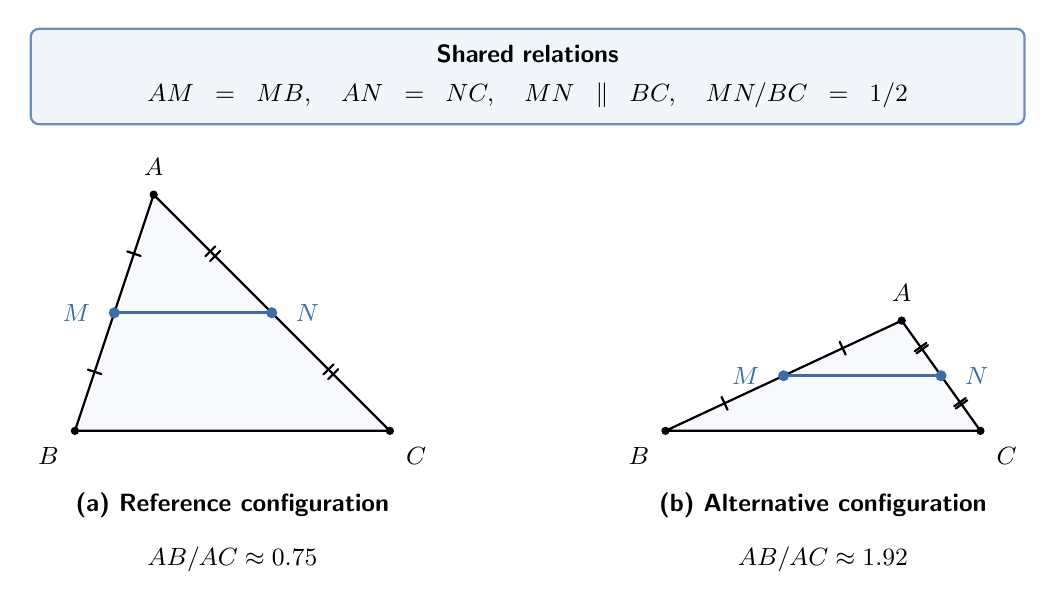
\begin{tikzpicture}[x=1cm,y=1cm,line width=.8pt,line cap=round,line join=round,font=\small]
\node[draw=borderPrimary,fill=bgPrimary!55,rounded corners=3pt,
text width=12.2cm,align=center,inner sep=6pt] at (5.75,4.5)
{\sffamily\textbf{Shared relations}\\[3pt]
$AM=MB,\quad AN=NC,\quad MN\parallel BC,\quad MN/BC=1/2$};
\foreach \dx/\ax/\ay/\panelLetter/\panelTitle/\ratio in
{0/1/3/a/{Reference configuration}/0.75,
7.5/3/1.4/b/{Alternative configuration}/1.92}{
\begin{scope}[shift={(\dx,0)}]
\path[use as bounding box] (-.6,-1.8) rectangle (4.6,3.5);
\coordinate (A) at (\ax,\ay);
\coordinate (B) at (0,0);
\coordinate (C) at (4,0);
\coordinate (M) at ($(A)!0.5!(B)$);
\coordinate (N) at ($(A)!0.5!(C)$);
\fill[bgPrimary!35] (A)--(B)--(C)--cycle;
\draw (A)--(B)--(C)--cycle;
\draw[borderAccent,line width=1.2pt] (M)--(N);
\foreach \t in {.25,.75}{
  \coordinate (T) at ($(A)!\t!(B)$);
  \draw ($(T)!0.09cm!90:(B)$)--($(T)!0.09cm!-90:(B)$);
}
\foreach \t in {.24,.26,.74,.76}{
  \coordinate (T) at ($(A)!\t!(C)$);
  \draw ($(T)!0.09cm!90:(C)$)--($(T)!0.09cm!-90:(C)$);
}
\foreach \P in {A,B,C}{\fill (\P) circle[radius=1.5pt];}
\foreach \P in {M,N}{\fill[borderAccent] (\P) circle[radius=2pt];}
\node[above=3pt] at (A) {$A$};
\node[below left=3pt] at (B) {$B$};
\node[below right=3pt] at (C) {$C$};
\node[left=5pt,text=borderAccent] at (M) {$M$};
\node[right=5pt,text=borderAccent] at (N) {$N$};
\node[anchor=north,align=center,text width=4.9cm,
font=\small\sffamily\bfseries,inner sep=2pt] (panelcaption) at (2,-.7)
{(\panelLetter) \panelTitle};
\node[align=center,inner sep=2pt,below=2mm of panelcaption]
{$AB/AC\approx\ratio$};
\end{scope}
}
\end{tikzpicture}
\caption[Different triangle shapes preserving midpoint relations]{Hai tam giác không đồng dạng giữ cùng các quan hệ trung điểm và đường trung bình. Khi đỉnh $A$ thay đổi, $M,N$ được dựng lại theo định nghĩa; các dấu trên cạnh biểu thị $AM=MB$ và $AN=NC$. Đoạn $MN$ màu xanh vẫn song song với $BC$ và có độ dài bằng một nửa $BC$, trong khi tỉ số $AB/AC$ thay đổi rõ rệt.}
\label{fig:valid-configurations}
\end{figure}


\paragraph{Quan hệ không gian trong biểu diễn 2D}

Với phép chiếu affine $\pi(P)=LP+t$ từ $\mathbb R^3$ xuống $\mathbb R^2$, các tổ hợp affine được bảo toàn:

\begin{equation}
\pi\!\left(\sum_i\alpha_iP_i\right)
=\sum_i\alpha_i\pi(P_i),
\qquad \sum_i\alpha_i=1.
\end{equation}

Đẳng thức suy ra bằng cách phân phối $L$ và sử dụng $\sum_i\alpha_i=1$ cho thành phần tịnh tiến. Vì vậy, quan hệ trung điểm, thuộc đoạn, song song và vector bằng nhau có thể được kiểm tra trên hình chiếu khi các đối tượng liên quan không bị suy biến.

Ví dụ, hình chiếu của lăng trụ có thể được xác định bởi $A,B,C,d\in\mathbb R^2$ với $A'=A+d$, $B'=B+d$, $C'=C+d$. Nếu $M=B+d/2$, $N=C+d/2$, $H=2B-A$ và $K=2C-A$, ta luôn có

\begin{equation}
2M=B+B'=A'+H,\qquad
2N=C+C'=A'+K.
\end{equation}

Các hệ thức này vẫn đúng khi thay đổi những điểm tự do. Bộ đánh giá do đó có thể kiểm tra các phụ thuộc được biểu diễn bằng điểm 2D mà không cần khôi phục toàn bộ tọa độ XYZ. Tuy nhiên, phép chiếu không khả nghịch: với $v\ne0$ thuộc $\ker L$, $\pi(P+v)=\pi(P)$. Các quan hệ đã kiểm tra trên hình chiếu không xác định duy nhất độ dài, góc hoặc cấu trúc không gian ẩn của vật thể.

\section{Dataset}
\label{sec:dataset}
\subsection{Data sources and scope}
Dữ liệu được tổ chức thành ba tác vụ Generate, Edit và Reconstruct. Generate và Edit sử dụng các yêu cầu hình học được biên soạn từ nguồn đã tuyển chọn, trong đó corpus SGK/SGV lớp 6--12 thuộc bộ \emph{Kết nối tri thức với cuộc sống} cung cấp phát biểu, mathematical givens và ngữ cảnh dựng hình. Các ví dụ, luyện tập và bài tập được xem như đơn vị nội dung hoàn chỉnh, bao gồm các tiểu ý xác định thêm đối tượng hoặc đường phụ. Taxonomy hình học gồm 17 mã G01--G17 được sử dụng trong khâu tuyển chọn và phân tích độ bao phủ nguồn.

Reconstruct sử dụng các cặp ảnh--TikZ từ snapshot Geo3K-TikZ \cite{geo3ktikz}. Trong bản export này, ảnh đầu vào là \texttt{rendered\_image} của nguồn, còn target giữ mã TikZ tương ứng. Do đó, nhánh Reconstruct cung cấp supervision cho ánh xạ từ hình đã render sang chương trình đồ họa; nguồn dữ liệu này được phân biệt với các bài toán SGK/SGV dùng để biên soạn Generate và Edit.

\subsection{Dataset statistics}
Bảng~\ref{tab:dataset-splits} trình bày số bản ghi của chín tệp Parquet trong bản export. Tổng cộng có 5,501 bản ghi, gồm 3,002 Reconstruct, 1,510 Generate và 989 Edit. Train, validation và test lần lượt chứa 3,470, 623 và 1,408 bản ghi. Các số liệu được xác định từ số hàng của tệp, không phải số bài toán hoặc cấu hình hình học duy nhất.

\begin{table}[tbp]
\centering
\caption[Dataset size by task and split]{Số bản ghi theo tác vụ và split trong bản export Hugging Face.}
\label{tab:dataset-splits}
\begin{tabular}{lrrrr}
\toprule
\textbf{Task} & \textbf{Train} & \textbf{Validation} & \textbf{Test} & \textbf{Total}\\
\midrule
Reconstruct & 1,467 & 375 & 1,160 & 3,002\\
Generate & 1,208 & 151 & 151 & 1,510\\
Edit & 795 & 97 & 97 & 989\\
\midrule
\textbf{Total} & \textbf{3,470} & \textbf{623} & \textbf{1,408} & \textbf{5,501}\\
\bottomrule
\end{tabular}
\end{table}

Nhánh Reconstruct giữ các bản ghi trùng từ nguồn và chứa 2,238 định danh ảnh khác nhau. Một bản ghi trong train split thiếu ảnh đầu vào; bản ghi này được tính trong Bảng~\ref{tab:dataset-splits} nhưng cần loại khi chuẩn bị image-to-TikZ training, còn 1,466 mẫu Reconstruct train có ảnh. Số bản ghi export vì vậy được phân biệt với số mẫu đủ đầu vào cho từng cấu hình huấn luyện.

\subsection{Record format and provenance}
Bản export sử dụng ba configurations tương ứng với tác vụ. Mỗi configuration có các tệp train, validation và test riêng; các trường đầu vào được giữ theo định nghĩa tác vụ tại Mục~\ref{sec:tasks}. Bảng~\ref{tab:dataset-fields} mô tả schema thực tế. Trong Generate, \texttt{current\_tikz} có giá trị null ở toàn bộ bản ghi. Trong Edit, trường này chứa mã của hình trước khi chỉnh sửa. Reconstruct lưu ảnh trực tiếp trong Parquet và không có trường instruction riêng; yêu cầu khôi phục được quy định ở task template.

\begin{table}[tbp]
\centering
\caption[Task-specific fields in the dataset export]{Các trường dữ liệu theo tác vụ. Mọi configuration đều có \texttt{id} và \texttt{target\_tikz}.}
\label{tab:dataset-fields}
\begin{tabularx}{\linewidth}{lXX}
\toprule
\textbf{Task} & \textbf{Input fields} & \textbf{Target}\\
\midrule
Generate & \texttt{instruction}; \texttt{current\_tikz} = null & \texttt{target\_tikz}\\
Edit & \texttt{instruction}, \texttt{current\_tikz} & \texttt{target\_tikz}\\
Reconstruct & \texttt{image} (embedded image bytes) & \texttt{target\_tikz}\\
\bottomrule
\end{tabularx}
\end{table}

Provenance đầy đủ được giữ trong hồ sơ chuẩn bị dữ liệu ngoại tuyến. Các bản ghi synthetic liên kết với bài toán nguồn, source family và những bản ghi Generate/Edit có liên quan. Export dùng cho huấn luyện chỉ giữ các trường cần thiết; metadata nguồn, lịch sử sửa và quyết định rà soát không trở thành context bổ sung cho mô hình. Với Reconstruct, \texttt{id} là SHA-256 của ảnh render nên các bản ghi dùng cùng ảnh có thể mang cùng định danh.

\subsection{Representative examples}
Các hình~\ref{fig:dataset-examples}--\ref{fig:dataset-reconstruct} minh họa ba tác vụ bằng các mẫu trong train split. Mỗi ví dụ trình bày input và target tương ứng: Generate nhận yêu cầu dựng hình; Edit nhận mã TikZ hiện tại và yêu cầu chỉnh sửa; Reconstruct nhận ảnh sơ đồ. Các render được tạo từ target trong dataset, không phải kết quả suy luận của mô hình đang được đánh giá.

\begin{figure}[htbp]
\centering
\begin{minipage}[t]{.47\linewidth}
\vspace{0pt}
\small\textbf{Drawing instruction}\par\medskip
Hình hộp ABCD.A'B'C'D'. Mặt phẳng song song với (ABB'A') cắt AD, BC, A'D', B'C' lần lượt tại M, N, M', N'. I là tâm của hình bình hành ABNM; J là tâm của hình bình hành A'B'N'M'. E là trung điểm của MN, E' là trung điểm của M'N'; EE' là đoạn thẳng nối hai trung điểm trong mặt phẳng (MNN'M').
\end{minipage}\hfill
\begin{minipage}[t]{.47\linewidth}
\vspace{0pt}
\centering\small\sffamily\textbf{Target TikZ render}\par\medskip
\resizebox{\linewidth}{!}{%
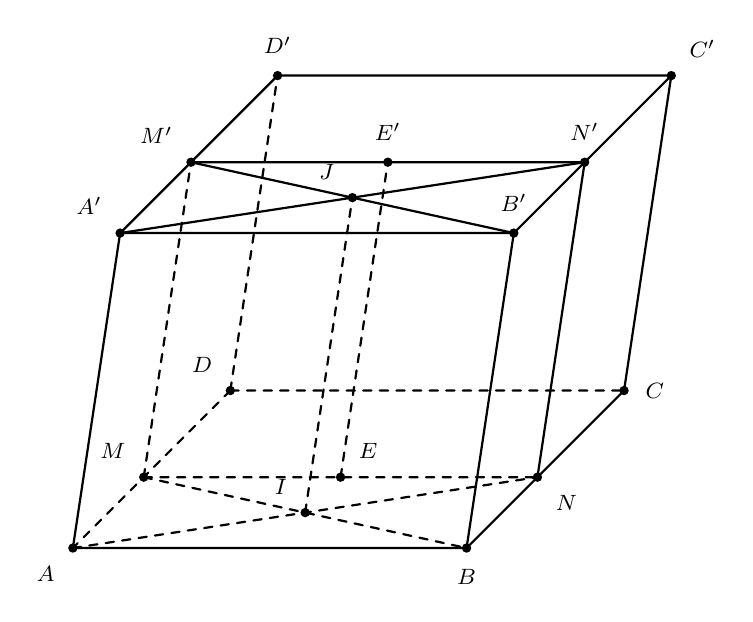
\begin{tikzpicture}[thick,line cap=round,line join=round,font=\footnotesize,label distance=2pt]
  \coordinate (A) at (0,0);
  \coordinate (B) at (5,0);
  \coordinate (D) at (2,2);
  \pgfmathsetmacro{\k}{0.45}

  \begin{pgfinterruptboundingbox}
  \coordinate (C) at ($(B)+(D)-(A)$);
  \coordinate (v) at (0.6,4.0);
  \coordinate (A') at ($(A)+(v)$);
  \coordinate (B') at ($(B)+(v)$);
  \coordinate (C') at ($(C)+(v)$);
  \coordinate (D') at ($(D)+(v)$);

  \coordinate (M) at ($(A)!\k!(D)$);
  \coordinate (N) at ($(B)!\k!(C)$);
  \coordinate (M') at ($(A')!\k!(D')$);
  \coordinate (N') at ($(B')!\k!(C')$);

  \coordinate (I) at ($(A)!0.5!(N)$);
  \coordinate (J) at ($(A')!0.5!(N')$);

  \coordinate (E) at ($(M)!0.5!(N)$);
  \coordinate (E') at ($(M')!0.5!(N')$);
  \end{pgfinterruptboundingbox}

  \draw[dashed] (D)--(C) (D)--(D') (D)--(M)--(A);
  \draw[dashed] (M)--(N) (M)--(M') (M)--(B) (A)--(N);
  \draw (A)--(B)--(N)--(C) (A)--(A') (B)--(B') (C)--(C');
  \draw (A')--(B')--(C')--(D')--cycle;
  \draw (M')--(N') (N)--(N');
  \draw (A')--(N') (B')--(M');
  \draw[dashed] (I)--(J);
  \draw[dashed] (E)--(E');

  \node[circle,fill,inner sep=1.2pt,label={below left:$A$}] at (A) {};
  \node[circle,fill,inner sep=1.2pt,label={below:$B$}] at (B) {};
  \node[circle,fill,inner sep=1.2pt,label={right:$C$}] at (C) {};
  \node[circle,fill,inner sep=1.2pt,label={above left:$D$}] at (D) {};
  \node[circle,fill,inner sep=1.2pt,label={above left:$A'$}] at (A') {};
  \node[circle,fill,inner sep=1.2pt,label={above:$B'$}] at (B') {};
  \node[circle,fill,inner sep=1.2pt,label={above right:$C'$}] at (C') {};
  \node[circle,fill,inner sep=1.2pt,label={above:$D'$}] at (D') {};

  \node[circle,fill,inner sep=1.2pt,label={above left:$M$}] at (M) {};
  \node[circle,fill,inner sep=1.2pt,label={below right:$N$}] at (N) {};
  \node[circle,fill,inner sep=1.2pt,label={above left:$M'$}] at (M') {};
  \node[circle,fill,inner sep=1.2pt,label={above:$N'$}] at (N') {};
  \node[circle,fill,inner sep=1.2pt,label={above left:$I$}] at (I) {};
  \node[circle,fill,inner sep=1.2pt,label={above left:$J$}] at (J) {};

  \node[circle,fill,inner sep=1.2pt,label={above right:$E$}] at (E) {};
  \node[circle,fill,inner sep=1.2pt,label={above:$E'$}] at (E') {};
\end{tikzpicture}
}
\end{minipage}
\caption[Generate example: a parallelepiped with auxiliary constructions]{Ví dụ Generate: từ yêu cầu dựng hình hộp, target biểu diễn thiết diện song song, tâm của hai hình bình hành và đoạn nối hai trung điểm. Instruction được giữ nguyên theo input trong dataset.}
\label{fig:dataset-examples}
\end{figure}

\begin{figure}[htbp]
\centering
\begin{minipage}[t]{.47\linewidth}
\vspace{0pt}
\centering\small\sffamily\textbf{Current TikZ render}\par\medskip
\resizebox{!}{5.2cm}{%
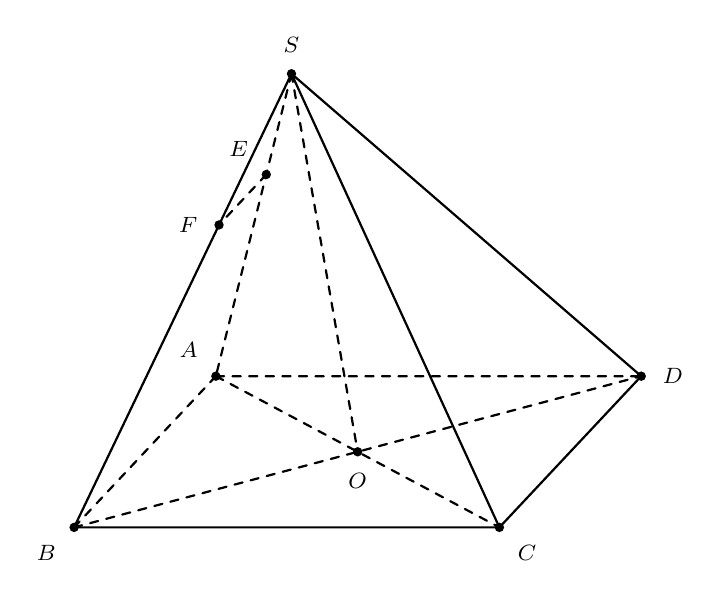
\begin{tikzpicture}[thick,line cap=round,line join=round,font=\footnotesize,label distance=2pt,scale=1.2]
  \coordinate (A) at (0,0);
  \coordinate (B) at (-1.5,-1.6);
  \coordinate (C) at (3,-1.6);
  \coordinate (D) at ($(A)+(C)-(B)$);
  \coordinate (S) at (0.8,3.2);

  \begin{pgfinterruptboundingbox}
  \path
    (intersection of A--C and B--D) coordinate (O)
    ($(S)!1/3!(A)$) coordinate (E)
    ($(S)!1/3!(B)$) coordinate (F);
  \end{pgfinterruptboundingbox}

  \draw[dashed] (A) -- (D) (A) -- (B) (S) -- (A) (A) -- (C) (B) -- (D) (S) -- (O) (E) -- (F);
  \draw (S) -- (B) -- (C) -- (D) -- (S) -- (C);

  \node[circle,fill,inner sep=1.2pt,label={above left:$A$}] at (A) {};
  \node[circle,fill,inner sep=1.2pt,label={below left:$B$}] at (B) {};
  \node[circle,fill,inner sep=1.2pt,label={below right:$C$}] at (C) {};
  \node[circle,fill,inner sep=1.2pt,label={right:$D$}] at (D) {};
  \node[circle,fill,inner sep=1.2pt,label={above:$S$}] at (S) {};
  \node[circle,fill,inner sep=1.2pt,label={below:$O$}] at (O) {};
  \node[circle,fill,inner sep=1.2pt,label={above left:$E$}] at (E) {};
  \node[circle,fill,inner sep=1.2pt,label={left:$F$}] at (F) {};
\end{tikzpicture}
}
\end{minipage}\hfill
\begin{minipage}[t]{.47\linewidth}
\vspace{0pt}
\centering\small\sffamily\textbf{Target TikZ render}\par\medskip
\resizebox{!}{5.2cm}{%
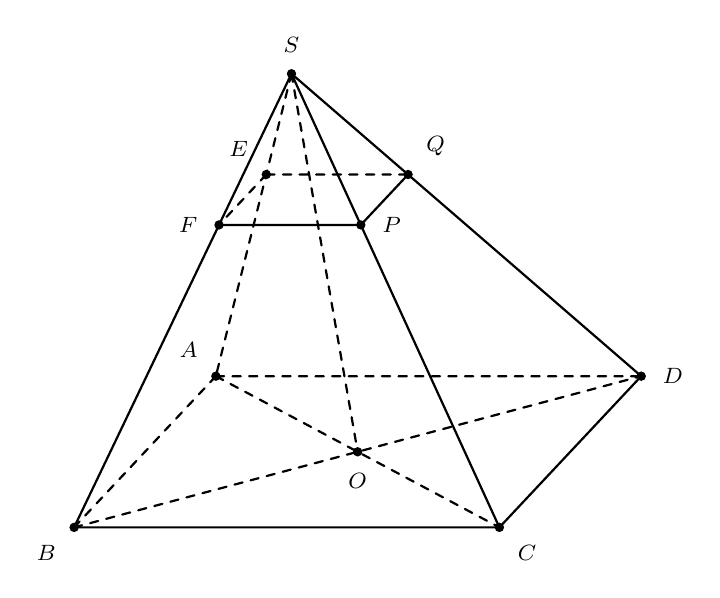
\begin{tikzpicture}[thick,line cap=round,line join=round,font=\footnotesize,label distance=2pt,scale=1.2]
  \coordinate (A) at (0,0);
  \coordinate (B) at (-1.5,-1.6);
  \coordinate (C) at (3,-1.6);
  \coordinate (D) at ($(A)+(C)-(B)$);
  \coordinate (S) at (0.8,3.2);

  \begin{pgfinterruptboundingbox}
  \path
    (intersection of A--C and B--D) coordinate (O)
    ($(S)!1/3!(A)$) coordinate (E)
    ($(S)!1/3!(B)$) coordinate (F)
    ($(S)!1/3!(C)$) coordinate (P)
    ($(S)!1/3!(D)$) coordinate (Q);
  \end{pgfinterruptboundingbox}

  \draw[dashed] (A) -- (D) (A) -- (B) (S) -- (A) (A) -- (C) (B) -- (D) (S) -- (O) (E) -- (F) (E) -- (Q);
  \draw (S) -- (B) -- (C) -- (D) -- (S) -- (C);
  \draw (F) -- (P) -- (Q);

  \node[circle,fill,inner sep=1.2pt,label={above left:$A$}] at (A) {};
  \node[circle,fill,inner sep=1.2pt,label={below left:$B$}] at (B) {};
  \node[circle,fill,inner sep=1.2pt,label={below right:$C$}] at (C) {};
  \node[circle,fill,inner sep=1.2pt,label={right:$D$}] at (D) {};
  \node[circle,fill,inner sep=1.2pt,label={above:$S$}] at (S) {};
  \node[circle,fill,inner sep=1.2pt,label={below:$O$}] at (O) {};
  \node[circle,fill,inner sep=1.2pt,label={above left:$E$}] at (E) {};
  \node[circle,fill,inner sep=1.2pt,label={left:$F$}] at (F) {};
  \node[circle,fill,inner sep=1.2pt,label={right:$P$}] at (P) {};
  \node[circle,fill,inner sep=1.2pt,label={above right:$Q$}] at (Q) {};
\end{tikzpicture}
}
\end{minipage}
\par\bigskip
\begin{minipage}{\linewidth}
\small\textbf{Edit instruction}\par\smallskip
P thuộc đoạn SC, Q thuộc đoạn SD sao cho SP = 1/3 SC, SQ = 1/3 SD; tứ giác EFPQ là thiết diện song song với đáy.
\end{minipage}
\caption[Edit example: completing a parallel cross-section of a pyramid]{Ví dụ Edit: hình chóp $S.ABCD$ và đoạn $EF$ đã có trong current TikZ (trái). Target (phải) bổ sung $P$, $Q$ cùng các cạnh $FP$, $PQ$, $QE$ để hoàn thiện thiết diện $EFPQ$ song song với đáy.}
\label{fig:dataset-edit}
\end{figure}

\begin{figure}[htbp]
\centering
\begin{minipage}[t]{.47\linewidth}
\vspace{0pt}
\centering\small\sffamily\textbf{Input diagram image}\par\medskip
\resizebox{\linewidth}{!}{\DatasetReconstructImage}
\end{minipage}\hfill
\begin{minipage}[t]{.47\linewidth}
\vspace{0pt}
\centering\small\sffamily\textbf{Target TikZ render}\par\medskip
\resizebox{\linewidth}{!}{%
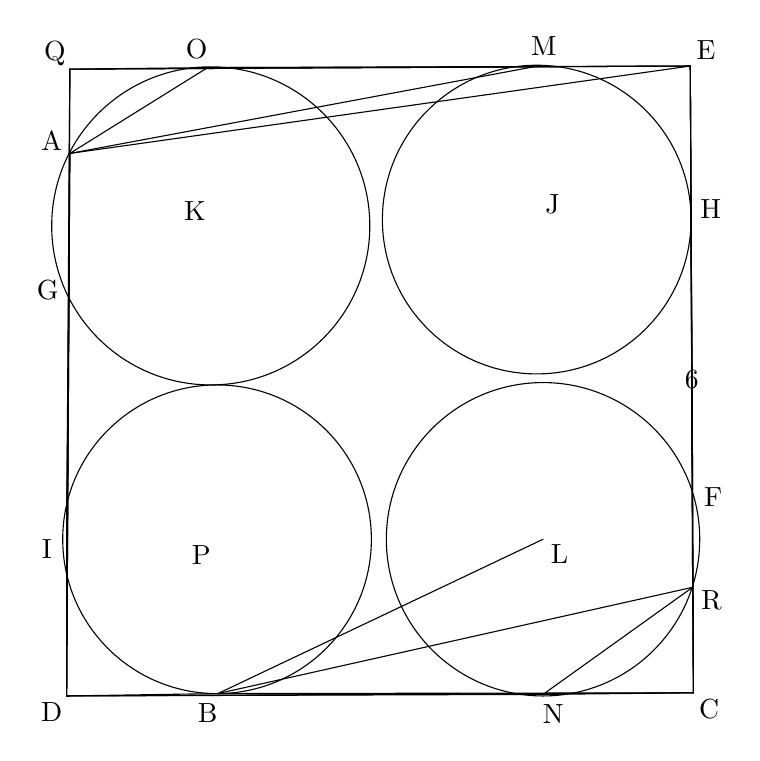
\begin{tikzpicture}[scale=1, line join=round, line cap=round]

    \coordinate (A) at (0.84, 7.69);
    \coordinate (B) at (2.72, 0.83);
    \coordinate (C) at (8.76, 0.84);
    \coordinate (D) at (0.80, 0.80);
    \coordinate (E) at (8.72, 8.80);
    \coordinate (F) at (8.75, 3.42);
    \coordinate (G) at (0.83, 5.87);
    \coordinate (H) at (8.73, 6.85);
    \coordinate (I) at (0.80, 2.78);
    \coordinate (J) at (6.77, 6.85);
    \coordinate (K) at (2.63, 6.77);
    \coordinate (L) at (6.85, 2.79);
    \coordinate (M) at (6.73, 8.79);
    \coordinate (N) at (6.85, 0.82);
    \coordinate (O) at (2.59, 8.78);
    \coordinate (P) at (2.71, 2.79);
    \coordinate (Q) at (0.84, 8.76);
    \coordinate (R) at (8.75, 2.18);

    \draw (J) circle (1.96);
    \draw (K) circle (2.02);
    \draw (L) circle (1.99);
    \draw (P) circle (1.96);

    \draw (A) -- (D);
    \draw (A) -- (E);
    \draw (A) -- (G);
    \draw (A) -- (I);
    \draw (A) -- (M);
    \draw (A) -- (O);
    \draw (A) -- (Q);
    \draw (B) -- (L);
    \draw (B) -- (N);
    \draw (C) -- (B);
    \draw (C) -- (F);
    \draw (C) -- (N);
    \draw (C) -- (R);
    \draw (D) -- (B);
    \draw (D) -- (C);
    \draw (D) -- (G);
    \draw (D) -- (I);
    \draw (D) -- (N);
    \draw (D) -- (Q);
    \draw (E) -- (C);
    \draw (E) -- (F);
    \draw (E) -- (H);
    \draw (E) -- (M);
    \draw (E) -- (O);
    \draw (E) -- (Q);
    \draw (E) -- (R);
    \draw (F) -- (R);
    \draw (G) -- (I);
    \draw (G) -- (Q);
    \draw (H) -- (C);
    \draw (H) -- (F);
    \draw (H) -- (R);
    \draw (I) -- (Q);
    \draw (M) -- (O);
    \draw (M) -- (Q);
    \draw (O) -- (Q);
    \draw (R) -- (B);
    \draw (R) -- (N);

    \node at (0.61, 7.85) {A};
    \node at (2.59, 0.58) {B};
    \node at (8.96, 0.64) {C};
    \node at (0.61, 0.60) {D};
    \node at (8.92, 9.00) {E};
    \node at (9.01, 3.33) {F};
    \node at (0.56, 5.95) {G};
    \node at (8.98, 6.98) {H};
    \node at (0.55, 2.66) {I};
    \node at (6.97, 7.05) {J};
    \node at (2.43, 6.96) {K};
    \node at (7.06, 2.60) {L};
    \node at (6.86, 9.05) {M};
    \node at (6.98, 0.57) {N};
    \node at (2.45, 9.02) {O};
    \node at (2.51, 2.59) {P};
    \node at (0.65, 8.96) {Q};
    \node at (8.99, 2.02) {R};

    \node at ($(E)!0.5!(C)$) {$6$};
\end{tikzpicture}
}
\end{minipage}
\caption[Reconstruct example: a diagram with four circles]{Ví dụ Reconstruct: input là ảnh sơ đồ chứa bốn đường tròn, các đoạn thẳng và nhãn (trái); target TikZ khôi phục các thành phần tương ứng (phải).}
\label{fig:dataset-reconstruct}
\end{figure}

\subsection{Data splits and quality control}
Generate và Edit được chia đồng thời theo các nhóm liên kết, với mục tiêu xấp xỉ 80/10/10 cho train, validation và test. Các nhóm được xác định từ source family, nguồn cha, quan hệ giữa bản ghi và mã TikZ trùng khớp. Toàn bộ nhóm được gán cùng split, vì vậy số lượng thực tế có thể lệch nhẹ khỏi tỷ lệ mục tiêu. Quy trình dùng seed 20261009 và lưu các quyết định chia để giữ ổn định giữa các lần export.

Reconstruct khởi đầu từ splits của nguồn Geo3K-TikZ. Những bản sao liên kết qua ảnh hoặc mã được gom cùng nhóm; khi một nhóm xuất hiện ở nhiều splits, việc gán ưu tiên test, rồi validation, rồi train. Các splits sau export vì vậy được xem là splits của bộ dữ liệu trong báo cáo, thay vì đồng nhất với benchmark gốc. Báo cáo export ghi nhận không có source-family links hoặc bản sao chính xác đi qua các splits; kết quả này không xác nhận sự vắng mặt của những mẫu gần trùng về ý nghĩa.

Kiểm tra export xác nhận các trường dữ liệu được giữ nguyên qua quá trình ghi và đọc Parquet. Chất lượng toán học và sự phù hợp giữa input--target được rà soát theo quy trình tại Mục~\ref{sec:data-curation}. Số lượng trong Bảng~\ref{tab:dataset-splits} mô tả quy mô bản export, không thay thế bằng chứng rà soát nội dung hoặc kết quả evaluation của mô hình.


\section{Experiments and Results}

\section{Discussion}
\label{sec:discussion}
\subsection{Implications for model training}
TikZ tạo một đích huấn luyện có thể chỉnh sửa và thực thi. Tuy nhiên, một đáp án tham chiếu chỉ là một cách hiện thực hóa dữ kiện. Khi dùng evaluation cho lựa chọn dữ liệu hoặc phản hồi huấn luyện, cần giữ sự khác biệt giữa đúng các quan hệ quan sát được và phù hợp với toàn bộ instruction. Điểm cao trên một target không thay thế bước kiểm tra chất lượng cặp input--target.

Việc tách metrics cho phép xác định phần cần cải thiện trong mô hình và quy trình. Compile failure liên quan đến khả năng viết mã; mất quan hệ hoặc nội dung liên quan đến diễn giải cấu hình; collision liên quan đến đặt nhãn và bố cục. Các scores có thể hỗ trợ phân tích hoặc thiết kế tín hiệu huấn luyện về sau, nhưng hiệu quả của việc sử dụng chúng làm reward cần được kiểm chứng bằng thực nghiệm riêng.

\subsection{Scope and limitations}

Phương pháp áp dụng cho các điểm có nhãn, đoạn thẳng nét liền hoặc đứt, đường tròn đầy đủ và dấu góc vuông được hỗ trợ bởi bước trích xuất. Các mã phân loại Gxx không thay đổi quy tắc tính điểm. Cung tổng quát, conic, miền tô và các điều kiện độ dài hoặc góc chỉ được mô tả bằng văn bản chưa được bao quát đầy đủ. Đối tượng chưa được hỗ trợ có thể làm giảm cả Content coverage và Visual readability.

Quan hệ được suy ra từ target có thể bao gồm những tính chất ngẫu nhiên của cách dựng, trong khi một điều kiện trong đề bài có thể không quan sát được trên hình. Vì vậy, $M=100$ chỉ có nghĩa là toàn bộ đơn vị quan hệ đã trích xuất đều đạt; tính phù hợp giữa target và bài toán là điều kiện tiên quyết. Các chứng minh bất biến ở trên áp dụng cho quan hệ hình học chính xác, còn kết quả tính điểm còn phụ thuộc vào trích xuất, liên kết nhãn và sai số số học.

Các phần trăm phản ánh tỉ lệ đơn vị đạt, không phải xác suất hình hoàn toàn đúng hoặc mức độ nghiêm trọng của lỗi. Visual readability chỉ đo va chạm và cắt nhãn trong phạm vi hỗ trợ, chưa thay thế đánh giá bố cục, tính thẩm mỹ hoặc hiệu quả sư phạm. Bốn chỉ số vì vậy được báo cáo riêng để giữ rõ ý nghĩa của từng khía cạnh chất lượng.

\section{Conclusion}
\label{sec:conclusion}
Báo cáo trình bày một hướng xây dựng hình vẽ hình học có thể chỉnh sửa bằng TikZ cho Generate, Edit và Reconstruct trong phạm vi lớp 6--12. Quy trình kết hợp chuẩn bị dữ liệu có nguồn, generation trực tiếp và kiểm tra ngoại tuyến từ kết quả thực thi. PDF đóng góp nội dung đã hiển thị; PGF hỗ trợ xác định vị trí gắn nhãn; các phép kiểm tra tất định tạo ra bốn metrics riêng.

Cơ sở hình học của evaluation cho phép đối chiếu quan hệ thay vì khớp tọa độ tuyệt đối. Uniform scaling, tịnh tiến, quay và phản xạ giữ các quan hệ được xét; nhiều cấu hình không đồng dạng cũng có thể hợp lệ khi các phụ thuộc còn được bảo toàn. Với hình không gian, các quan hệ affine biểu diễn trên hình chiếu có thể được kiểm tra bằng điểm 2D trong điều kiện không suy biến.

Bước tiếp theo là hoàn thiện targets đã duyệt, tổ chức held-out data theo source family và thực hiện so sánh mô hình theo protocol đã xác định. Việc mở rộng checks cho các đối tượng ngoài phạm vi hiện tại và đánh giá mức phù hợp với instruction cần đi cùng bằng chứng kiểm chứng. Những kết quả đó sẽ quyết định khả năng sử dụng quy trình trong huấn luyện và tái sử dụng hình toán học ở quy mô lớn.

\clearpage
\phantomsection
\addcontentsline{toc}{section}{\refname}
\begin{thebibliography}{99}

\bibitem{automat} Belouadi, J., Lauscher, A., và Eger, S. \emph{AutomaTikZ: Text-Guided Synthesis of Scientific Vector Graphics with TikZ}. ICLR, 2024. \href{https://arxiv.org/abs/2310.00367}{arXiv:2310.00367}.

\bibitem{mathematikz} Malik, R., Hao, R. L., Kacholia, R., và Demszky, D. \emph{MathemaTikZ: A Benchmark for K-12 Mathematical Diagram Generation}. 2025. \href{https://www.dorademszky.com/publications/49731.pdf}{Author manuscript}.

\bibitem{tikzilla} Greisinger, C., và Eger, S. \emph{TikZilla: Scaling Text-to-TikZ with High-Quality Data and Reinforcement Learning}. ICLR, 2026. \href{https://arxiv.org/abs/2603.03072}{arXiv:2603.03072}.

\bibitem{ref1} Belouadi, J. và cộng sự. \emph{TikZero: Zero-Shot Text-Guided Graphics Program Synthesis}. 2025. Mục 5, Evaluation Metrics. \href{https://arxiv.org/html/2503.11509v1#S5}{arXiv:2503.11509v1}.

\bibitem{magicgeo} Wang, J. và cộng sự. \emph{MagicGeo: Training-Free Text-Guided Geometric Diagram Generation}. 2025. \href{https://arxiv.org/abs/2502.13855}{arXiv:2502.13855}.

\bibitem{ref3} Wei, X. và cộng sự. \emph{GeoLoom: High-quality Geometric Diagram Generation from Textual Input}. arXiv:2512.08180v2, 2026. Mục 3–4. \href{https://arxiv.org/html/2512.08180v2#S4.SS2}{Bản gốc}.

\bibitem{detikzify} Belouadi, J., Ponzetto, S. P., và Eger, S. \emph{DeTikZify: Synthesizing Graphics Programs for Scientific Figures and Sketches with TikZ}. NeurIPS, 2024. \href{https://arxiv.org/abs/2405.15306v3}{arXiv:2405.15306v3}.

\bibitem{geobridge} Sun, J. và cộng sự. \emph{GeoTikzBridge: Advancing Multimodal Code Generation for Geometric Perception and Reasoning}. CVPR, 2026. \href{https://arxiv.org/abs/2603.22687}{arXiv:2603.22687}.

\bibitem{edit2tikz} Zhang, Z. và cộng sự. \emph{Edit2TikZ: A Comprehensive and Challenging Benchmark for Scientific Figure Editing with TikZ}. Preprint, 2026. \href{https://arxiv.org/abs/2608.13441v1}{arXiv:2608.13441v1}.

\bibitem{editikz} Greisinger, C., Zhao, Z., và Eger, S. \emph{EdiTikZ: Scientific Figure Editing from Revision Trajectories}. Preprint, 2026. \href{https://arxiv.org/abs/2609.01409v2}{arXiv:2609.01409v2}.

\bibitem{ref2} Kumar, V. và cộng sự. \emph{DiagramIR: An Automatic Pipeline for Educational Math Diagram Evaluation}. 2025. Mục 2.2–2.3. \href{https://arxiv.org/html/2511.08283v1#S2.SS3}{arXiv:2511.08283v1}.

\bibitem{ref4} \emph{PGF/TikZ Manual}, mục Transformations. \href{https://tikz.dev/tikz-transformations}{Official documentation}.

\bibitem{geminiflash} Google. \emph{What's new in Gemini 3.8 Flash}. Gemini API documentation. \href{https://ai.google.dev/gemini-api/docs/latest-model?hl=en}{Official documentation}.

\bibitem{qwen35} Qwen Team. \emph{Qwen3.5-4B: Model Card}. \href{https://huggingface.co/Qwen/Qwen3.5-4B}{Official model card}.

\bibitem{unsloth35} Unsloth. \emph{Qwen3.5 Fine-tuning Guide}. \href{https://unsloth.ai/docs/models/qwen3.5/fine-tune}{Official documentation}.

\bibitem{lora} Hu, E. J. và cộng sự. \emph{LoRA: Low-Rank Adaptation of Large Language Models}. ICLR, 2022. \href{https://arxiv.org/abs/2106.09685}{arXiv:2106.09685}.
\bibitem{mineru} OpenDataLab. \emph{MinerU}. \href{https://github.com/opendatalab/MinerU}{Official repository}.

\bibitem{react} Yao, S., Zhao, J., Yu, D., Du, N., Shafran, I., Narasimhan, K., và Cao, Y. \emph{ReAct: Synergizing Reasoning and Acting in Language Models}. 2023. \href{https://arxiv.org/abs/2210.03629v3}{arXiv:2210.03629v3}.


\bibitem{geo3ktikz} SunnyLin. \emph{Geo3K-TikZ}. Hugging Face dataset. \href{https://huggingface.co/datasets/SunnyLin/geo3k-tikz/tree/main}{Dataset repository}.

\end{thebibliography}
\end{document}
